\newpage
\pagestyle{fancy}
\chapter*{Aceleraci\'on estoc\'astica de part\'iculas en una fulguraci\'on solar}
\addcontentsline{toc}{chapter}{Aceleraci\'on estoc\'astica de part\'iculas en una fulguraci\'on solar}



\renewcommand{\baselinestretch}{1.0}

\begin{wrapfigure}[29]{r}{0.46\textwidth}
\begin{center}
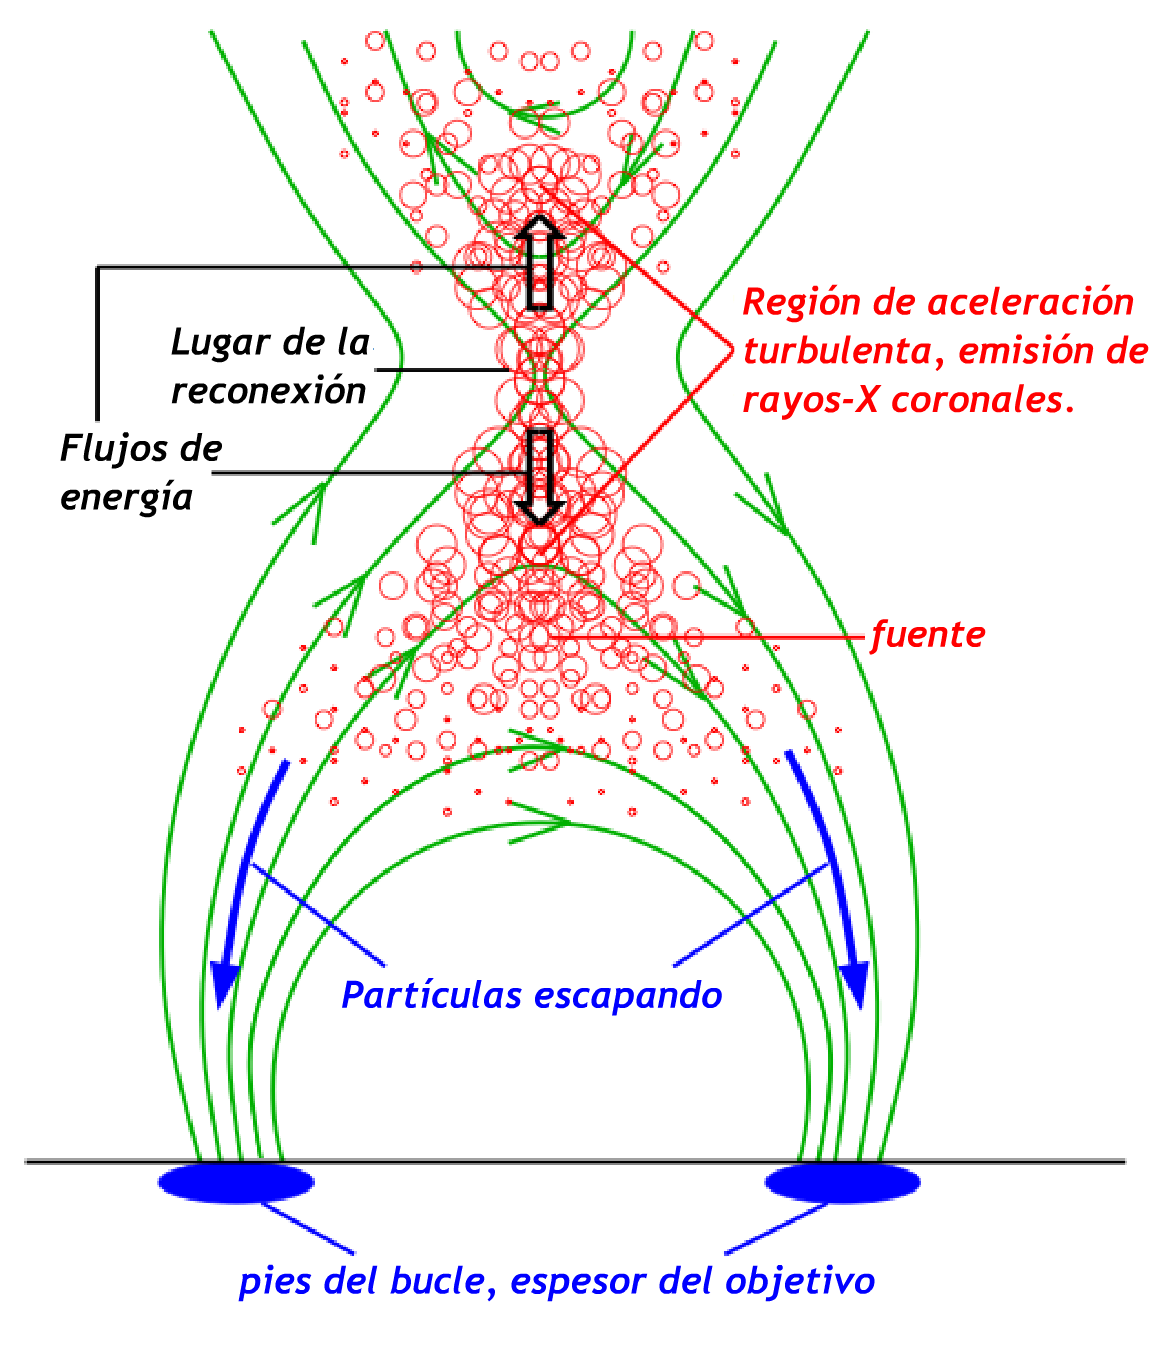
\includegraphics[width=0.39\textwidth]{wei-liu.png}
\caption{Esquema del modelo de aceleraci\'on estoc\'astica propuesto para las fulguraciones solares. Las curvas en verde representan las l\'ineas de campo magn\'etico en una configuraci\'on posible; los c\'irculos en rojo representan la turbulencia o las ondas del plasma que se generan durante el evento de la fulguraci\'on. {\it Tomado y modificado de} \citep[]{liu2008}.}
\label{fig:liu}
\end{center}
\end{wrapfigure}

En el estudio de las fulguraciones solares se trabaja b\'asicamente con tres mecanismos diferentes de aceleraci\'on de part\'iculas: (1) {\bf Aceleraci\'on directa por acci\'on de un campo el\'ectrico}: \citep[]{HOLMAN1985,wood2005} Se plantea que la aceleraci\'on del {\it jet}\footnote{Usamos aqu\'i el t\'ermino en ingl\'es {\it jet} para referirnos a un haz de part\'iculas tipo chorro, para estar m\'as acorde con la nomenclatura internacional al respecto.} de part\'iculas cargadas se lleva a cabo mediante una aplicaci\'on sencilla de una fuerza tipo Coulomb mediante un campo el\'ectrico DC que se genera sobre la zona de reconexi\'on; el problema m\'as grande que sobrelleva este modelo es la dificultad de mantenerlo a gran escala. (2) {\bf Aceleraci\'on de Fermi a primer orden (choque)}: \citep[]{Tsuneta1998} Este mecanismo plantea que la manera en la que se les suministra energ\'ia a las part\'iculas es cuando son embestidas por un frente de una onda de choque producto de un hipot\'etico {\it jet super-magnetos\'onico} proveniente de la regi\'on de reconexi\'on. Adem\'as, este proceso deja ver escalas de tiempo del orden de los 0.3 - 0.6 s que est\'an de acuerdo con las observaciones. Aunque esta din\'amica ofrece una explicaci\'on plausible de la inyecci\'on de las part\'iculas hacia el interior solar, tiene algunos problemas en cuanto a las consecuencias que traer\'ia sobre las part\'iculas que saldr\'ian expelidas hacia el espacio interplanetario. (3) {\bf Aceleraci\'on estoc\'astica o aceleraci\'on de Fermi a segundo orden}: La turbulencia y las ondas de plasma son los eventos m\'as comunes que est\'an presentes cuando se da un evento de fulguraci\'on solar \citep[]{petrosian1994,miller1998}. En el modelo de {\it aceleraci\'on estoc\'astica} el esquema b\'asico de la din\'amica propuesta es como la que se presenta en la figura \ref{fig:liu}. 

Como una consecuencia de la reconexi\'on magn\'etica bien sea mediante la turbulencia a gran escala o bien mediante las ondas de plasma que son generadas cerca del punto-X de reconexi\'on, las part\'iculas son aceleradas, y estas, a su vez, producen una emisi\'on en rayos-X duros que se producen cerca de la cima del bucle de la fulguraci\'on en el llamado {\it thin target}, como producto de una emisi\'on t\'ermica por parte de las part\'iculas  aceleradas. El registro de esta emisi\'on ha sido uno de los mayores logros de la misi\'on {\it Yohkoh}. Las part\'iculas que no son atrapadas en la cima y que logran escapar hacia la parte baja de la atm\'osfera solar, al interactuar con el plasma que rodea los pies del bucle, emiten tambi\'en en rayos-X duros por radiaci\'on {\it Bremsstrahlung} y forman los conocidos {\it thick target} en las vecindades de los {\it footpoints}.\\

Este mecanismo ha sido profundamente estudiado por diversos autores no solamente en el marco del estudio de las fulguraciones solares sino en varias otras ramas de la astrof\'isica que involucran este tipo de procesos como en los agujeros negros, en los {\it Gamma Ray Burts} (GRB), los n\'ucleos activos de galaxias, etc \citep[]{park1996,1996miller,1997park,Liu2004A}.\\


Usualmente cuando en f\'isica se habla de un proceso estoc\'astico se debe hacer referencia a la ecuaci\'on de {\it Boltzmann}. Pues bien, trabajos desarrollados por \cite{F1914} y \cite{P1917} a principios del siglo pasado mostraron todo un desarrollo en cuanto a la teor\'ia existente detr\'as de un proceso de aceleraci\'on estoc\'astica de un ensamble de part\'iculas puntuales con la posibilidad de poder introducir en este formalismo diferentes interacciones entre ellas y fuerzas externas a ellas. Gracias a esto, hoy en d\'ia esta ecuaci\'on se conoce como la ecuaci\'on de {\it Fokker-Planck}, la cual ser\'a el tema de la siguiente secci\'on.


\section*{Ecuaci\'on de Fokker-Planck}
\addcontentsline{toc}{section}{Ecuaci\'on de Fokker-Planck}

La ecuaci\'on de {\it Fokker-Planck} b\'asicamente brinda un formalismo que permite estudiar la din\'amica de un sistema de muchas part\'iculas en el cual los efectos de las colisiones entre ellas cobran una importancia relevante en el planteamiento de su din\'amica.\\

Hacia comienzos del siglo XX, y despu\'es de que Einstein hubiese propuesto su hip\'otesis del movimiento {\it browniano} en uno de sus famosos art\'iculos de 1905\footnote{En 1905 Albert Einstein public\'o su art\'iculo titulado: ``{\it \"{U}ber die von der molekularkinetischen Theorie der W\"arme geforderte Bewegung von in ruhenden Fl\"ussigkeiten suspendierten Teilchen}'' (Sobre la teor\'ia cin\'etica-molecular del calor requerido por el movimiento de part\'iculas suspendidas en l\'iquidos en reposo) en el {\it Annalen der Physik} en que planta las bases del atomismo moderno dando una explicaci\'on razonable del movimiento aleatorio que presentan part\'iculas peque\~nas suspendidas sobre un estanque de agua en reposo.}, se centraron muchos esfuerzos en analizar este ``curioso'' comportamiento de movimiento aleatorio que registraban las part\'iculas subat\'omicas. En busca de esto se desarrollaron una variedad de experimentos en los que por ejemplo se enfriaba Hidr\'ogeno l\'iquido hasta temperaturas muy cercanas al cero absoluto con el fin de observar el movimiento de un conjunto de semillas peque\~nas que se depositaban sobre su superficie. Al mismo tiempo, se trabajaba en desarrollos te\'oricos en aras de establecer un formalismo te\'orico que brindara explicaci\'on a este comportamiento; en este sentido fue {\it A.D. Fokker} quien en 1914 public\'o su trabajo titulado ``{\it Die mittlere Energie rotierender elektrischer Dipole im Strahlungsfeld}'' o  `` Energ\'ia media de rotaci\'on de dipolos el\'ectricos inmersos en un campo de radiaci\'on'', en el cual por primera vez muestra un tratamiento estoc\'astico con el objetivo de ligar este comportamiento aleatorio de naturaleza microsc\'opica con variables observables a nivel macrosc\'opico \citep[]{F1914}. Tres a\~nos m\'as tarde, {\it Planck} recoge y complementa los trabajos de {\it Fokker} y publica un art\'iculo en el que formaliza una ecuaci\'on que trabaja con la din\'amica de las part\'iculas involucradas en el espacio de fases y construye un formalismo regido por una mec\'anica de fluidos en dicho espacio que facilita mucho su descripci\'on \citep[]{P1917}. Es por esto que hoy d\'ia a dicha ecuaci\'on se le conoce con el nombre {\bf ecuaci\'on de Fokker-Planck}.\\

Existen varias formas de introducir la ecuaci\'on de {\it Fokker-Planck}; una de ellas es a trav\'es del uso de un formalismo {\it browniano} que incluya t\'erminos colisionales para dar pie a una deducci\'on natural y simplificada de dicha expresi\'on. La forma m\'as general se encuentra al eliminar toda restricci\'on sobre los fen\'omenos que puedan influir el movimiento del sistema de part\'iculas. Este desarrollo como muchas aplicaciones a diferentes sistemas f\'isicos est\'a muy bien explicado por \cite{risken}. Una presentaci\'on m\'as formal que tiene en cuenta los postulados de la mec\'anida cu\'antica y la mec\'anica estad\'istica se encuentra en los trabajos desarrollados por \cite{chandra1943}. 

\subsection*{Un primer acercamiento: la ecuaci\'on de Langevin}
\addcontentsline{toc}{subsection}{Un primer acercamiento: la ecuaci\'on de Langevin}

Empezamos considerando un sistema de muchas part\'iculas que se mueven aleatoriamente. Centramos nuestra atenci\'on en una de ellas cuya masa $m$ es apreciablemente mayor que la del resto de part\'iculas y la cual se encuentra inmersa en este sistema, {\it i.e.} est\'a bajo la influencia de la din\'amica asociada a dicho ensamble. En general, la fuerza que siente esta part\'icula es proporcional a la velocidad que \'esta tenga dentro del fluido:

\begin{align}
\mathbf{F}=-\alpha\mathbf{v}
\end{align}

\noindent haciendo uso de la segunda ley de Newton podemos reescribir esto como:

\begin{align}
m\dot{\mathbf{v}}+\alpha\mathbf{v}=0\\
\dot{\mathbf{v}}+\gamma\mathbf{v}=0
\end{align}

\noindent donde $\gamma\equiv \alpha/m=1/\tau$, siendo $\tau$ el tiempo caracter\'istico de decaimiento de la fuerza. Esta ecuaci\'on tiene soluci\'on exacta cuando se conoce el valor de $\mathbf{v}$ para un tiempo inicial $t_0$:

\begin{align}\label{determ}
\mathbf{v}(t)=\mathbf{v}(t_0)\exp(-t/\tau)=\mathbf{v}(t_0)\exp(-\gamma t).
\end{align}

Detr\'as de esta fuerza viscosa lo que se encuentra es que las part\'iculas que conforman el sistema f\'isico en estudio colisionan con la part\'icula de inter\'es present\'andose una transferencia de momentum que es el responsable de que la velocidad de la part\'icula poco a poco vaya decreciendo hasta hacerse cero. Pero n\'otese un aspecto importante; la ecuaci\'on (\ref{determ}) es una expresi\'on determinista, lo que significa que supone que para un tiempo arbitrario $t$ el valor de la velocidad de la part\'icula est\'a completamente definida siempre y cuando se hayan establecido las condiciones iniciales apropiadamente, pero esto solo puede ser cierto si la masa $m$ de la part\'icula de inter\'es es lo suficientemente grande comparada con la del resto de part\'iculas que conforman el ensamble de manera que las fluctuaciones t\'ermicas de la velocidad puedan ser despreciadas.\\

Del teorema de equipartici\'on de la energ\'ia, la energ\'ia de la part\'icula es (en una dimensi\'on)

\begin{align}
\frac{1}{2}m\langle v^2\rangle=\frac{1}{2}kT,
\end{align}

\noindent siendo $k$ la  constante y $T$ la temperatura. Ahora bien, si la masa llega a ser peque\~na entonces la ecuaci\'on (\ref{determ}) deja de ser v\'alida. \'Esta ecuaci\'on debe ser modificada para introducir correctamente los efectos que la energ\'ia t\'ermica tiene sobre la din\'amica de esta peque\~na part\'icula. La modificaci\'on consiste en introducir una fuerza de tipo estoc\'atico $\mathbf{F}_f(t)$ en donde estar\'ian contenidos todos los efectos de la din\'amica molecular asociada al medio de propagaci\'on. As\'i,

\begin{align}
\dot{\mathbf{v}}+\gamma\mathbf{v}=\mathbf{\Gamma}(t),
\end{align}

\noindent siendo $\mathbf{\Gamma}(t)=\mathbf{F}_f(t)/m$, en donde $\mathbf{F}_f(t)$ se conoce como la fuerza de {\it Langevin}. Hay varias suposiciones que se establecen sobre el $\mathbf{\Gamma}(t)$, la primera es que su promedio sobre todo el ensamble debe ser cero,

\begin{align}
\langle\mathbf{\Gamma}(t)\rangle=0,
\end{align}

\noindent ya que el promedio sobre sobre las velocidades $\langle\mathbf{v}(t)\rangle$ debe satisfacer la ecuaci\'on (\ref{determ}). Adem\'as, si se multiplican dos fuerzas de {\it Langevin} correspondientes a tiempos distintos $t$ y $t'$ cuya diferencia es apreciablemente mayor que el tiempo caracter\'istico de colisi\'on $\tau_c$ y se hace el promedio sobre todo el ensamble, este promedio tambi\'en debe ser nulo:

\begin{align}\label{eq:gamma}
\langle\mathbf{\Gamma}(t)\mathbf{\Gamma}(t')\rangle=0\quad\text{para}\quad |t-t'|\geq \tau_c
\end{align}

\noindent que puede ser re-escrita tomando el l\'imite cuando $\tau_c\rightarrow 0$, pues en ese caso se set\'a localizando temporalmente en $t=t'$. De este modo, en lugar de la ecuaci\'on (\ref{eq:gammag}) tenemos:

\begin{align}
\langle\mathbf{\Gamma}(t)\mathbf{\Gamma}(t')\rangle=q\delta(t-t').
\end{align}

Como vemos es importante entender la dependencia temporal de variables aleatorias para estar en la capacidad de construir una descripci\'on completa de este tipo de din\'amicas, y es en esa direcci\'on que se trabaja a continuaci\'on.

\subsection*{Dependencia temporal de variable aleatorias y deducci\'on de la ecuaci\'on de Fokker-Planck unidimensional}
\addcontentsline{toc}{subsection}{Deducci\'on de la ecuaci\'on de Fokker-Planck unidimensional}

\renewcommand{\baselinestretch}{1.0}

\begin{wrapfigure}[13]{r}{0.54\textwidth}
\begin{center}
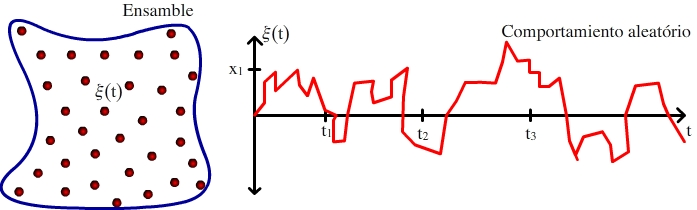
\includegraphics[width=0.5\textwidth]{aleatorio.jpg}
\caption{Esquematizaci\'on de un ensamble de sistemas f\'isicos que tiene asociado a \'el una cierta cantidad $\xi$ que se comporta de manera aleatoria con el tiempo.}
\label{fig:aleatorio}
\end{center}
\end{wrapfigure}

Comencemos considerando un ensamble de muchas part\'iculas en cuya din\'amica interviene una cantidad que var\'ia aleatoriamente y que es representada por la letra $\xi$. Supongamos adem\'as que esa cantidad $\xi$ depende del tiempo de forma tal que pueda describirse como una funci\'on de $t$, $\xi(t)$, tal como se representa en la figura \ref{fig:aleatorio}. En imposible predecir con absoluta certeza el comportamiento que mostrar\'a $\xi$ con el transcurrir del tiempo. Se acude entonces a lo que se acostumbra a hacer en estos casos y es trabajar con densidades de probabilidad.\\

Definimos la densidad de probabilidad de que $\xi(t_1)$ se encuentre entre el intervalo $x_1\leq\xi(t_1)\leq x_1+dx_1$, en donde $x_1\,\epsilon\,D(\xi)$, siendo $D(\xi)$ el conjunto dominio de los valores de $\xi$.

\begin{align}
W_1(x_1,t_1)=\langle\delta(x_1-\xi(t_1))\rangle,
\end{align}

\noindent donde con los s\'imbolos  $\langle\rangle$ se expresa un promedio sobre todo el ensamble. Ahora bien, en esta misma v\'ia se puede definir la densidad de probabilidad de que $\xi(t_1)$ se encuentre en el intervalo $x_1\leq\xi(t_1)\leq x_1+dx_1$ pero que tambi\'en $\xi(t_2)$ est\'e en $x_2\leq\xi(t_2)\leq x_2+dx_2$, ..., y que  $\xi(t_n)$ est\'e contenido en $x_n\leq\xi(t_n)\leq x_n+dx_n$ como

\begin{align}
W_n(x_n,t_n;...;x_1,t_1)=\langle\delta(x_1-\xi(t_1))...\delta(x_n-\xi(t_n))\rangle.
\end{align}

Supongamos ahora que conocemos una cierta cantidad de densidades de probabilidad jerarquizadas como sigue:

\begin{align}
&W_1(x_1,t_1)\\\nonumber
&W_2(x_1,t_1;x_2,t_2)\\\nonumber
&W_3(x_1,t_1;x_2,t_2;x_3,t_3)\\\nonumber
&...
\end{align}

\noindent para todo $t_i$ que se encuentre en el intervalo $t_0\leq t_i\leq t_0+T$. En otras palabras, lo que esto indica es suponer que se conoce la evoluci\'on temporal completa de la variable aleatoria $\xi(t)$. \\

La exigencia de conocer estas densidades de probabilidad de manera expl\'icita se hace con fin de poder definir formalmente los valores promedios de ciertas cantidades propias del sistema f\'isico bajo una simple integral, i.e. poderlas correlacionar entre s\'i. Por ejemplo, siendo $t'>t$, la correlaci\'on de la variable aleatoria entre dos diferentes tiempos se puede expresar como

\begin{align}
\langle\xi(t)\,\xi(t')\rangle=\int x\,...\,x'W'(x,t;...;x',t')\,dx\,...\,dx'.
\end{align}

{\bf Densidad de probabilidad restringida} (o condicionada): Basados en lo anterior podemos definir una densidad de probabilidad de la variable aleatoria $\xi$ para un tiempo $t_n$ bajo la condici\'on de que para un $t_{n-1}<t_n$ se tenga a certeza de que la variable aleatoria tom\'o el valor $x_{n-1}$, para $t_{n-2}<t_{n-1}$, $\xi(t_{n-2})=x_{n-2}$, y as\'i sucesivamente hasta que para $t_1<t_2$, $\xi(t_1)=x_1$. Formalmente,

\begin{align}
P(x_n,t_n|x_{n-1},t_{n-1};...;x_1,t_1)=\langle\delta(x_n-\xi(t_n))\rangle|_{\xi(t_{n-1})=x_{n-1},...,\xi_{t_1}=x_1}.
\end{align}\\

Esta misma densidad de probabilidad restringida se puede expresar en funci\'on de los $W_n$ como:

\begin{align}\label{pxn}
P(x_n,t_n|x_{n-1},t_{n-1};...;x_1,t_1)=\frac{W_n(x_n,t_n;...;x_1,t_1)}{W_{n-1}(x_{n-1},t_{n-1};...;x_1,t_1)},
\end{align}

\noindent pero dado que $W_{n-1}$ la podemos re-escribir como

\begin{align}
W_{n-1}(x_{n-1},t_{n-1};...;x_1,t_1)=\int W_n(x_n^*,t_n^*;...;x_1,t_1)\,dx_n^*,
\end{align}

\noindent (\ref{pxn}) toma la forma

\begin{align}
P(x_n,t_n|x_{n-1},t_{n-1};...;x_1,t_1)=\frac{W_n(x_n,t_n;...;x_1,t_1)}{\int W_n(x_n^*,t_n^*;...;x_1,t_1)\,dx_n^*};
\end{align}

\noindent de donde finalmente se deduce que

\begin{align}\label{wp}
W_n(x_n,t_n;...;x_1,t_1)=\int P(x_n,t_n|x_{n-1},t_{n-1};...;x_1,t_1)\,W_n(x_n^*,t_n^*;...;x_1,t_1)\,dx_n^*.
\end{align}\\

En general; si definimos un $x'=x+\varepsilon$, con $\varepsilon>0$, y como $t+\tau>t$, con $\tau>0$; podemos re-escribir (\ref{wp}) como

\begin{align}\label{wxt}
W(x',t+\tau)=\int P(x',t+\tau|x,t)\,W(x,t)\,dx,
\end{align}

\noindent siendo $P(x',t+\tau|x,t)$ la densidad de probabilidad de que ocurra la transici\'on de $x,\,t$ a $x',\,t+\tau$. Ahora bien, en la ecuaci\'on de {\it Fokker-Planck} interviene la derivada temporal de $W(x,t)$, $\partial W(X,T)/\partial t$, para lo cual es inherente conocer la probabilidad de transici\'on $P(x',t+\tau|x,t)$ para valores de $\tau$ peque\~nos, y en busca de una representaci\'on de esta derivada es que se trabaja a continuaci\'on.\\

Para empezar establecemos la suposici\'on de que es posible conocer todos los {\bf momentos} estad\'isticos de la distribuci\'on, esto es, que se conoce

\begin{align}
M_n(x,t,\tau)=\langle[\xi(t+\tau)-\xi(t)]^n\rangle |_{\xi(t)=x}=\int (x'-x)^nP(x',t+\tau|x,t)\,dt
\end{align}

\noindent para todo $n\,\epsilon\,\mathds{Z}$. Ahora bien, podemos hacer uso de la siguiente identidad general de los {\it deltas de Dirac}:

\begin{align}\label{pxp}
P(x',t+\tau|x,t)=\int\delta(y-x')\,P(y,t+\tau|x,t)\,dy,
\end{align}

\noindent y expresar $\delta(y-x')$ como $\delta(y-x+x-x')$.\\

Ahora, tratemos de expandir la funci\'on {\it delta de Dirac} en series de Taylor. La expresi\'on general para una expanci\'on en series de Taylor es

\begin{align}
f(x^*-x_0^*)=\sum_{n=0}^{\infty}\frac{f^{(n)}(x_0^*)}{n!}(x^*-x_0^*)^n.
\end{align}

\noindent Si, para nuestro caso, $x^*=(y-x)$, y, $x_0^*=(x'-x)$, as\'i

\begin{align}
\delta(y-x')&=\sum_{n=0}^\infty \frac{(y-x')^n}{n!}\left(\frac{\partial}{\partial x^*}\right)^n\delta(x'-x)\\\label{delta}
&=\sum_{n=0}^\infty \frac{(y-x')^n}{n!}\left(-\frac{\partial}{\partial x}\right)^n\delta(x'-x).
\end{align}

Introduciendo (\ref{delta}) en (\ref{pxp}) se tiene

\begin{align}
P(x',t+\tau|x,t)=\int\sum_{n=0}^\infty \frac{(y-x')^n}{n!}\left(-\frac{\partial}{\partial x}\right)^n\delta(x'-x)\,P(y,t+\tau|x,t)\,dy,
\end{align}

\noindent que sacando el primer t\'ermino de la suma se convierte en

\begin{align}
P(x',t+\tau|x,t)=\int\delta(x'-x)\,P(y,t+\tau|x,t)\,dy+\int\sum_{n=1}^\infty\frac{(y-x')^n}{n!}\left(-\frac{\partial}{\partial x}\right)^n\delta(x'-x)\,P(y,t+\tau|x,t)\,dy,
\end{align}

\noindent reacomodando t\'erminos:

\begin{align}
P(x',t+\tau|x,t)=\delta(x'-x)\,\underbrace{\int P(y,t+\tau|x,t)\,dy}_{\text{identidad}}+\sum_{n=1}^\infty\frac{1}{n!}\left(-\frac{\partial}{\partial x}\right)^n\delta(x'-x)\underbrace{\int(y-x)^n\,P(y,t+\tau|x,t)\,dy}_{M_n(x,t,\tau)},
\end{align}

\begin{align}
P(x',t+\tau|x,t)&=\delta(x-x')+\sum_{n=1}^\infty\frac{1}{n!}\left(-\frac{\partial}{\partial x}\right)^n\delta(x'-x)\,M_n(x,t,\tau),\\
&=\left[1+\sum_{n=1}^\infty\frac{1}{n!}\left(-\frac{\partial}{\partial x}\right)^n\,M_n(x,t,\tau)\right]\,\delta(x-x'),
\end{align}

\noindent donde se ha tenido en cuenta la identidad $\delta(x-x')=\delta(x'-x)$.\\

Insertando este \'ultimo resultado en (\ref{wxt}), tenemos

\begin{align}
W(x',t+\tau)&=\int P(x',t+\tau|x,t)\,W(x,t)\,dx\\
&=\int \left[1+\sum_{n=1}^\infty\frac{1}{n!}\left(-\frac{\partial}{\partial x}\right)^n\,M_n(x,t,\tau)\right]\,\delta(x-x')\,W(x,t)\,dx\\\label{ww}
&=W(x',t)+\sum_{n=1}^\infty\frac{1}{n!}\left(-\frac{\partial}{\partial x}\right)^n\int\delta(x-x')\,M_n(x,t,\tau)W(x,t)\,dx.
\end{align}

Por otro lado, cuando se considera el l\'imite en el que $\tau<<1$ 

\begin{align}
W(x',t+\tau)-W(x',t)=\frac{\partial W(x',t)}{\partial t}+\sigma(\tau^2),
\end{align}

\noindent en donde $\sigma(\tau^2)$ representa t\'erminos de orden superior a $\tau^2$; de esta manera, de (\ref{ww}) se tiene que

\begin{align}
W(x',t+\tau)-W(x',t)&=\sum_{n=1}^\infty\frac{1}{n!}\left(-\frac{\partial}{\partial x}\right)^n\int\delta(x-x')\,M_n(x,t,\tau)W(x,t)\,dx\\
\frac{\partial W(x',t)}{\partial t}&=\frac{1}{\tau}\sum_{n=1}^\infty\frac{1}{n!}\left(-\frac{\partial}{\partial x}\right)^n\int\delta(x-x')\,M_n(x,t,\tau)\,W(x,t)\,dx\\\label{wt}
&=\sum_{n=1}^\infty\frac{1}{n!}\left(-\frac{\partial}{\partial x'}\right)^n\,M_n(x',t,\tau)\,W(x',t).
\end{align}

Si se define $D^{(n)}(x',t)\equiv\frac{M_n(x',t,\tau)}{\tau\,(n!)}$, entonces (\ref{wt}) se generaliza como

\begin{align}
\boxed{\frac{\partial W(x',t)}{\partial t}=\sum_{n=1}^\infty\left(-\frac{\partial}{\partial x'}\right)^n\,D^{(n)}(x',t)\,W(x',t)}
\end{align}

\noindent que es la llamada {\it ecuaci\'on general de Kramer-Moyal} en una dimensi\'on.\\

Cuando la serie de {\it Kramer-Moyal} se trunca a segundo orden obtenemos la ecuaci\'on general de {\it Fokker-Planck} unidimensional:

\begin{align}
\boxed{\frac{\partial W(x,t)}{\partial t}=-\frac{\partial}{\partial x}[D^{(1)}(x,t)\,W(x,t)]+\frac{\partial^2}{\partial x^2}[D^{(2)}(x,t)\,W(x,t)]}
\end{align}

\subsection*{Ecuaci\'on de Fokker-Planck Multi-dimensional}
\addcontentsline{toc}{subsection}{Ecuaci\'on de Fokker-Planck Multi-dimensional}

Empecemos considerando un sistema de $N$ variables aleatorias $\{\xi\}=\{\xi_1,\xi_2,...,\xi_N\}$ para lograr extender la ecuaci\'on (\ref{wxt}) a 

\begin{align}\label{ro}
W(\{x'\},t+\tau)=\int P(\{x'\},t+\tau|\{x\},t)\,W(\{x\},t)\,d^Nx, 
\end{align}

\noindent donde el elemento de volumen es $d^Nx=dx_1\,dx_2\,...\,dx_N$ y el s\'imbolo integral resume las $N$ integrales que se deben hacer. A\'i mismo, $\{x\}$, $\{x'\}$ arriba (ecuaci\'on \ref{ro}), y en lo que sigue de esta secci\'on, representa al conunto ordenado de las respectivas variables. La funci\'on {\it delta} para estas $N$ variables es

\begin{align}
\delta(\{x\})=\delta(x_1)\,\delta(x_2)\,...\,\delta(x_N),
\end{align}

\noindent con lo que 

\begin{align}\label{si}
P(\{x'\},t+\tau|\{x\},t)=\int\delta(\{y\}-\{x'\})\,P(\{y\},t+\tau|\{x\},t)\,d^Ny.
\end{align}

Ahora trabajemos sobre la funci\'on $\delta(\{y\}-\{x'\})$ expandiendola en series \citep[]{aguirre2000},

\begin{align}
\delta(\{y\}-\{x'\})&=\delta(\{x\}-\{x'\}+\{y\}-\{x\})\\
&=\sum_{\nu=0}^\infty\frac{1}{\nu!}(y_{j1}-x_{j1})(y_{j2}-x_{j2})...(y_{j\nu}-x_{j\nu})\frac{\partial^\nu}{\partial x_{j1}\,\partial x_{j2}\,...\,\partial x_{j\nu}}\delta(\{x\}-\{x'\})\\\label{au}
&=\sum_{\nu=0}^\infty\frac{1}{\nu!}\frac{(-\,\partial)^\nu}{\partial x'_{j1}\,\partial x'_{j2}\,...\,\partial x'_{j\nu}}(y_{j1}-x_{j1})(y_{j2}-x_{j2})...(y_{j\nu}-x_{j\nu})\delta(\{x\}-\{x'\}),
\end{align}

\noindent donde se ha usado la notaci\'on de {\it suma} sobre los \'indices repetidos. Insertando (\ref{au}) en (\ref{si}), tenemos

\begin{align}\label{mi}
P(\{x'\},t+\tau|\{x\},t)=\left[1+\sum_{\nu=1}^\infty\frac{1}{\nu!}\frac{(-\,\partial)^\nu}{\partial x_{j1}\,\partial x_{j2}\,...\,\partial x_{j\nu}}M_{j_1,j_2,...,j_\nu}^{(\nu)}(\{x\},t,\tau)\right]\delta(\{x'\}-\{x\}),
\end{align}

\noindent donde se ha usado la definici\'on de {\it $\nu$-\'esimo} momento estad\'istico como

\begin{align}
M_{j_1,j_2,...,j_\nu}^{(\nu)}(\{x\},t,\tau)=\int(y_{j1}-x_{j1})(y_{j2}-x_{j2})\, ....\,(y_{j\nu}-x_{j\nu})\,P(\{y\},t+\tau|\{x\},t)\,d^Ny.
\end{align}

Llevando (\ref{mi}) a (\ref{ro}),

\begin{align}
W(\{x'\},t+\tau)&=\int \left[1+\sum_{\nu=1}^\infty\frac{1}{\nu!}\frac{(-\,\partial)^\nu}{\partial x_{j1}\,\partial x_{j2}\,...\,\partial x_{j\nu}}M_{j_1,j_2,...,j_\nu}^{(\nu)}(\{x'\},t,\tau)\right]\delta(\{x'\}-\{x\})\,W(\{x\},t)\,d^Nx,\\
W(\{x'\},t+\tau)-W(\{x'\},t)&=\sum_{\nu=1}^\infty\frac{1}{\nu!}\frac{(-\,\partial)^\nu}{\partial x_{j1}\,\partial x_{j2}\,...\,\partial x_{j\nu}}\int \delta(\{x'\}-\{x\})\,M_{j_1,j_2,...,j_\nu}^{(\nu)}(\{x\},t,\tau)\,W(\{x\},t)\,d^Nx,\\\label{lale}
\frac{\partial W(\{x'\},t)}{\partial t}&=\frac{1}{\tau}\sum_{\nu=1}^\infty\frac{1}{\nu!}\frac{(-\,\partial)^\nu}{\partial x'_{j1}\,\partial x'_{j2}\,...\,\partial x'_{j\nu}}\,M_{j_1,j_2,...,j_\nu}^{(\nu)}(\{x'\},t,\tau)\,W(\{x'\},t),
\end{align}

\noindent siento $\tau$ el intervalo de tiempo infinitesimal transcurrido entre $t$ y $t+\tau$.\\

Si definimos $D_{j_1,j_2,...,j_\nu}^{(\nu)}(\{x\},t)=\frac{M_{j_1,j_2,...,j_\nu}^{(\nu)}(\{x\},t,\tau)}{\tau\,(\nu!)}$, entonces (\ref{lale}) toma la forma m\'as general

\begin{align}
\boxed{\frac{\partial W(\{x'\},t)}{\partial t}=\sum_{\nu=1}^\infty\frac{(-\,\partial)^\nu}{\partial x'_{j1}\,\partial x'_{j2}\,...\,\partial x'_{j\nu}}\,D_{j_1,j_2,...,j_\nu}^{(\nu)}(\{x'\},t)\,W(\{x'\},t),}
\end{align}

\noindent conocida como la {\it ecuaci\'on de Kramer-Moyal multidimensional}. Cuando truncamos esta serie a segundo orden obtenemos la famosa ecuaci\'on de {\it Fokker-Planck} en varias variables:

\begin{align}\label{efp}
\boxed{\frac{\partial W(\{x\},t)}{\partial t}=-\,\frac{\partial}{\partial x_{j_1}}\,D_{j_1}^{2}(\{x\},t)\,W(\{x\},t)+\frac{\partial^2}{\partial x_{j_1}\,\partial x_{j_2}}\,D_{j_1\,j_2}^{2}(\{x\},t)\,W(\{x\},t),}
\end{align}

\noindent donde se usa la notaci\'on de suma sobre \'indices repetidos.

\subsection*{Ecuaci\'on de Fokker-Planck para una distribuci\'on de electrones que se inyecta en un plasma magnetizado}
\addcontentsline{toc}{subsection}{Din\'amica de un paquete de electrones que se inyecta en un plasma magnetizado}

La aceleraci\'on de electrones a altas energ\'ias es un fen\'omeno que se presenta en m\'ultiples escenerios astrof\'isicos como en los rayos c\'osmicos, en los jets de rayos gamma, en los n\'ucleos activos de galaxias, en los eventos de supernova y en las fulguraciones solares \citep[]{longair1992}. Con el advenimiento de la era moderna de la tecnolog\'ia y gracias a la extrema cercan\'ia del Sol con respecto a nosotros ha sido posible obtener una gran cantidad de datos observacionales (espectros e im\'agenes) de alta resoluci\'on espacial y temporal. Estas observaciones posibilitan la comparaci\'on detallada de los datos de ciencia con un an\'alisis te\'orico de la evoluci\'on temporal de la distribuci\'on electr\'onica mediante el empleo adecuado de la ecuaci\'on de {\it Fokker-Planck} como ecuaci\'on cin\'etica de movimiento del proceso en estudio. Es clara entonces la importancia de establecer los par\'ametros f\'isicos del medio en el cual se propagar\'an los electrones en la formulaci\'on te\'orica.\\

\begin{wrapfigure}[25]{l}{0.54\textwidth}
\begin{center}
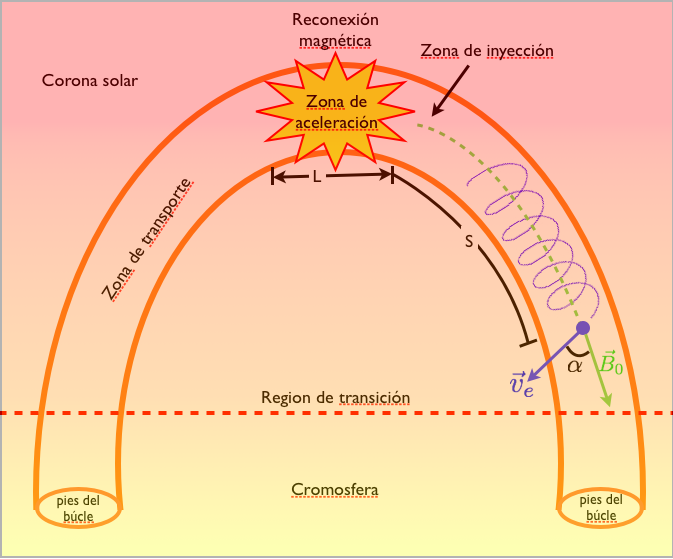
\includegraphics[width=0.53\textwidth]{pitchangle.png}
\caption{Esquematizaci\'on del giro-movimiento de una part\'icula cargada cuanto se transporta a lo largo de las l\'ineas de campo magn\'etico en el interior de un b\'ucle de plasma coronal.}
\label{fig:giromovimiento}
\end{center}
\end{wrapfigure}

B\'asicamente, durante las \'ultimas tres d\'ecadas se ha dado un avance importante en la construcci\'on de una descripci\'on te\'orica consistente que considere los procesos relevantes presentes en la interacci\'on del paquete de electrones en su viaje a trav\'es del plasma \citep[]{leach1981,bai1982,lu1988,mctiernan1990,hamilton1990,miller1996,1997park,liu2004,liu2009,zharkova2011a}.\\

Estos trabajos previos han mostrado que algunos de los procesos f\'isicos que causan que la distribuci\'on electr\'onica evolucione con el tiempo son la dispersi\'on {\it Coulombiana} y tipo {\it Compton}, la reflexi\'on magn\'etica, las interacciones tipo {\it onda-part\'icula}, la radiaci\'on sincrotr\'on, y los efectos directos de los campos el\'ectricos tipo DC, siendo los par\'ametros f\'isicos propios del plasma (tales como la densidad, la magnitud y topolog\'ia del campo magn\'etico y la energ\'ia y composici\'on de las part\'iculas) los factores que determinan cu\'ales de estos procesos predominan en el fen\'omeno.\\

La mayor\'ia de los plasmas astrof\'isicos se encuentran inmersos en un campo magn\'etico producto del movimiento de las part\'iculas cargadas que lo componen. Si en dichos plasmas la magnitud del campo magn\'etico predomina sobre la del campo el\'ectrico, el movimiento de las part\'iculas se hace principalmente a lo largo de las l\'ineas de $\vec{B}$ en lo que se conoce como {\it giro-movimiento} (ver figura \ref{fig:giromovimiento}). Este giro-movimiento se caracteriza por tres observables f\'isicos: la energ\'ia de la part\'icula en movimiento $E$, su posici\'on $s$, y el \'angulo de cabeceo $\alpha$; o en ingl\'es {\it pitch angle}, el cual se refiere al \'angulo formado entre el vector momentum de la part\'icula $\vec{p}$ en un instante dado y el vector campo magn\'etico $\vec{B}$ del lugar.\\

Si sobre uno de estos plasmas se inyecta un n\'muero grande de part\'iculas cargadas (por ejemplo electrones) con una distribuci\'on dada $W$, la din\'amica de estas, la evoluci\'on de sus movimientos, se podr\'a describir como se mostr\'o en la secci\'on anterior. En este caso, consideremos nuestra funci\'on de distribuci\'on $W$ como una funci\'on que depende de la energ\'ia $E$, la posici\'on de la part\'icula $s$ en la regi\'on, y del coseno del \'angulo de cabeceo $\mu$. As\'i, $W=W(E,\mu,s,t)$, y los c\'alculos pertinentes se llevar\'an a cabo en el espacio de fases. 

En este caso la ecuaci\'on de {\it Fokker-Planck} (\ref{efp}) toma la forma:

\begin{align}\label{eq:fph}
\frac{\partial W}{\partial t}=-\text{v}\mu\frac{\partial W}{\partial s}-\frac{\partial}{\partial \mu}(\dot{\mu}W)-\frac{\partial}{\partial E}(\dot{E}W)+\frac{\partial}{\partial\mu}\left(D_{\mu\mu}\frac{\partial W}{\partial\mu}\right)+\frac{\partial}{\partial E}\left(D_{EE}\frac{\partial W}{\partial E}\right)+\frac{\partial}{\partial E}\left(D_{E\mu}\frac{\partial W}{\partial\mu}\right)+\frac{\partial}{\partial\mu}\left(D_{E\mu}\frac{\partial W}{\partial E}\right).
\end{align}

Los coeficientes $\text{v}\cos\alpha$, $\dot{\mu}$ y $\dot{E}$ son los cambios sistem\'aticos en posici\'on, \'angulo de cabeceo y energ\'ia, respectivamente, producto de las fuerzas externas que act\'uan directamente sobre las part\'iculas en movimiento. Las cantidades $D_{j_1j_2}$ est\'an asociadas directamente con los diferentes procesos de dispersi\'on y por eso hacen parte de los t\'erminos difusivos de la expresi\'on \citep[]{hamilton1990}. Las formas expl\'icitas de los coeficientes $\dot{E}$, $\dot{\mu}$ y $D_{j_1j_2}$ para un conjunto de electrones bajo la influencia de colisiones tipo Coulomb, dispersiones Compton y de interacci\'on onda-part\'icula, radiaci\'on sincrotr\'on, variaciones del campo magn\'etico, y fuerzas externas son resumidas en las siguientes dos tablas \citep[]{hamilton1990}:

\begin{table}[htdp]
\caption{Tasas de cambio de la energ\'ia y el \'angulo de cabeceo. $\ln\Lambda$ es el logaritmo Coulombiano.}
\begin{center}
\begin{tabular}{|c|c|c|}\hline\hline
Proceso  & $\dot{E}$ & $\dot{\mu}$ \\\hline & & \\
Colisi\'on Coulombiana & $-4\pi ncr_0^2\ln\Lambda/\beta$ & 0 \\ & & \\
Emisi\'on sincrotr\'on & $-\frac{2}{3}B^2\gamma^2\beta^2(1-\mu^2)/mc$ & $-\frac{2}{3}r_0^2B^2\mu(1-\mu^2)/mc\gamma$ \\ & & \\
Fuerzas externas & $\mu\beta\,\mathbf{F}_{||}/mc$ & $(1-\mu^2)\mathbf{F}_{||}/\gamma\beta mc$ \\ & & \\
Reflejo magn\'etico & 0 & $-\frac{1}{2}\beta c(1-\mu^2)(d\ln B/ds)$ \\ & & \\
Ondas de Alfv\'en & $(1/\gamma\beta^2)(1-\beta^2)D_{EE}^{\text{Alfv\'en}}$ & $(1/\gamma\beta^2)(1+\beta^2)D_{E\mu}^{\text{Alfv\'en}}$ \\ & & \\
Ondas de Langmuir & $(1/\gamma\beta^2)(1-\beta^2)D_{EE}^{\text{Langmuir}}$ & 0 \\ & & \\\hline
\end{tabular}
\end{center}
\label{procesos}
\end{table}%

\begin{table}[htdp]
\caption{Coeficientes de difusi\'on}
\begin{center}
\begin{tabular}{|c|c|c|c|}\hline\hline
Coeficientes & Colisi\'on Coulombiana & Ondas de Alfv\'en & Ondas de Langmuir \\\hline & & & \\
$D_{\mu\mu}$ & $\frac{4\pi ncr_0^2\ln\Lambda}{\beta^2\gamma^2}(1-\mu^2)$ & $D_{-}^{(2)}+D_{+}^{(2)}$ & 0 \\ & & & \\
$D_{EE}$ & $\sim0$ & $\beta^4\gamma^2\frac{v_A^2}{v^2}(D_{-}^{(0)}+D_{+}^{(0)})$ & $\frac{ncr_0^2\epsilon_L}{\beta}\overline{k^{-3}}$ \\ & & & \\
$D_{E\mu}$ & $\sim0$ & $\beta^4\gamma^2\frac{v_A}{v}(D_{-}^{(1)}+D_{+}^{(1)})$ & 0 \\ & & & \\\hline
\end{tabular}
\end{center}
\label{difusion}
\end{table}%

En general, para la aceleraci\'on estoc\'astica de un conjunto de part\'iculas cargadas asociada a un proceso de fulguraci\'on solar, \cite{lu1988} mostraron que la ecuaci\'on (\ref{eq:fph}) toma la forma particular

\begin{align}\label{fph}
\frac{\lambda_0}{\text{v}}\frac{\partial W}{\partial t}=-\lambda_0\mu\frac{\partial W}{\partial s}+\lambda_0\frac{d\,\ln\,B}{ds}\frac{\partial}{\partial \mu}\left[\frac{(1-\mu^2)}{2}W\right]+\frac{c^2}{\text{v}}\frac{\partial}{\partial E}\left(\frac{W}{\text{v}}\right)+\frac{c^4}{\text{v}^4\gamma^2}\frac{\partial}{\partial \mu}\left[(1-\mu^2)\frac{\partial W}{\partial \mu}\right]+\frac{\lambda_0}{\text{v}}S(E,\mu,s,t),
\end{align}

\noindent donde $\lambda_0(s)=(10^{24\,\text{cm}})/n(s)\,\ln\Lambda$ es una cantidad que est\'a relacionada con el camino libre medio de un electr\'on que tienen una energ\'ia $E$  a trav\'es de la relaci\'on $\lambda(E)=\lambda_0\,E^2/(E+1)$. $n(s)$ es la densidad de n\'umero de part\'iculas del plasma en el ambiente en el cual se propaga el electr\'on.\\

Un an\'alisis completo y deductivo de modelamientos que se han hecho considerando algunos de estos tipos de interacciones se encuentran en \citep[]{petrosian1981,leach1981,petrosian1985,mctiernan1989,mctiernan1990,hamilton1990,somov1,ls1993,petrosian1994,Holman2001}. Sin embargo, en el cap\'itulo siguiente se muestra un revisi\'on ligera de los {\it tres} mecanismos que se consideran en el desarrollo del presente trabajo.\\

\section*{Procesos relevantes involucrados en las colisiones en plasmas}
\addcontentsline{toc}{section}{Procesos relevantes involucrados en las colisiones en plasmas}


\subsection*{Colisi\'on Coulombiana}
\addcontentsline{toc}{subsection}{Colisi\'on Coulombiana}

Tenemos que encargarnos de comprender cada una de las diferentes interacciones que se quieren considerar para el modelamiento de la interacci\'on del jet de electrones con el plasma de la atm\'osfera solar. El primer proceso que vemos en las tablas (\ref{procesos}) y (\ref{difusion}) es la colisi\'on entre part\'iculas tipo Coulomb. Esto se debe a que en general una part\'icula que incide velozmente sobre un plasma tiene colisiones con los electrones at\'omicos y con los n\'ucleos que lo componen. Los electrones del plasma, al ser ligeros, pueden adquirir una cantidad de energ\'ia apreciable por parte de los electrones incidentes sin provocar desviaciones importantes en la direcci\'on de su movimiento; mientras que, los n\'ucleos, de mayor masa, absorben muy poca energ\'ia; pero, en cambio, por efecto de su carga, provocan dispersiones notables a las part\'iculas incidentes. Una pregunta que se evidencia en las m\'ultiples explicaciones que se tratan de dar en cuanto al sistema de generaci\'on de sismos asociados a fulguraciones solares es: Si los electrones al poseer menor masa se ven m\'as alterados en su trayectoria y tienden a difundirse en su camino, c\'omo es que logran tener alcances tan profundos de la atm\'osfera solar para eventualmente estar asociados a la generaci\'on de la fuente s\'ismica? Este es uno de los mayores contra-argumentos que se dan al intentar de proponer un modelo como el nuestro, pero que algunos autores tratan de responder atribuyendo esta capacidad de penetraci\'on a la enorme cantidad de energ\'ia adquirida en el momento de la explosi\'on y posteriormente en el proceso de aceleraci\'on \citep[]{zharkova2011a}.\\

\begin{figure}[ht!]
\begin{center}
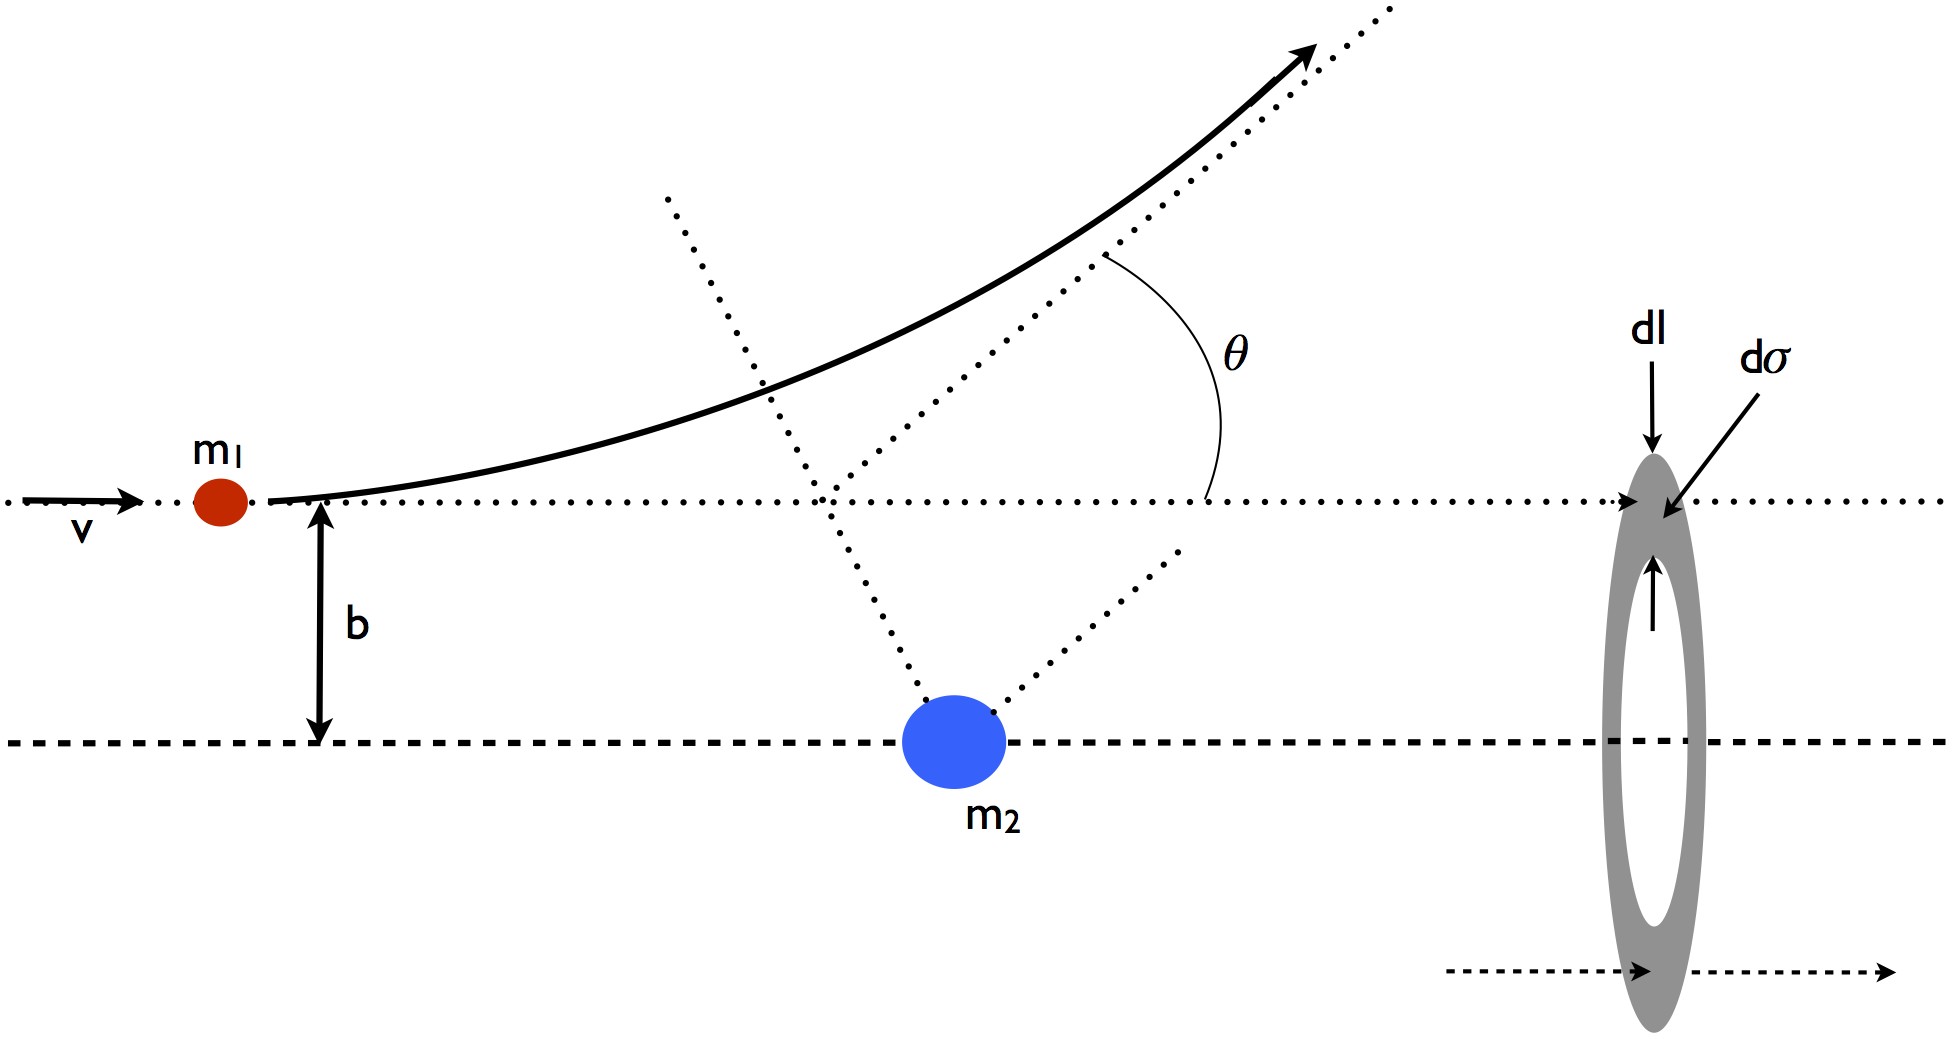
\includegraphics[width=0.73\textwidth]{coulomb.png}
\caption{Esquematizaci\'on de la interacci\'on de dos part\'iculas el\'ectricamente cargadas mediante un potencial {\it coulombiano}. Ilustraci\'on de los conceptos de par\'ametro de impacto y secci\'on eficaz.}
\label{fig:coulomb}
\end{center}
\end{figure}


La colisi\'on de dos part\'iculas relacionadas mediante un potencial {\it Coulombiano}, $\phi=e/r$, genera intercambios de momentum y de energ\'ia, y por tanto p\'erdidas cuando nos centramos en una part\'icula que incide sobre otra, ambas con una carga el\'ectrica asociada. Esta interacci\'on se esquematiza en la figura \ref{fig:coulomb}.\\

Si consideramos un sistema de referencia cuyo origen se encuentre en el centro de masa del sistema de las dos part\'iculas, cada una de las part\'iculas se dispersa un \'angulo $\theta$ definido por la relaci\'on

\begin{align}\label{theta1}
\tan\frac{\theta}{2}=\frac{e_1e_2}{\mu \text{v}^2b},
\end{align}

\noindent donde $\mu=\frac{m_1m_2}{m_1+m_2}$ es la masa reducida del sistema, $e_1$ y $e_2$ son las cargas respectivas de cada una de las part\'iculas, v es la velocidad inicial relativa de la part\'icula incidente y $b$ es el {\it par\'ametro de impacto} de la interacc\'on. Para ver una deducci\'on formal de la expresi\'on (\ref{theta1}) \citep[]{landau-mecanica}. Ahora bien, para una part\'icula que se deflecta un \'angulo de $\pi/2$

\begin{align}
b\left(\frac{\pi}{2}\right)=b_{\perp}=\frac{e_1e_2}{\mu \text{v}^2},
\end{align}

\noindent de manera que podemos escribir (\ref{theta1}) como

\begin{align}
\tan\frac{\theta}{2}=\frac{b_\perp}{b}.
\end{align}

Se habla entonces de una colisi\'on cercana si 

\begin{align}
\pi/2\leq\theta\leq\pi,\qquad\text{i.e.}\qquad0\leq b\leq b_\perp,
\end{align}

\noindent correspondientemente se tiene que, una colisi\'on lejana ser\'a aquella para la cual $b>b_\perp$ y $0\leq\theta\leq\pi/2$. Los dos casos pueden ser comprendidos a trav\'es de la figura \ref{fig:coulomb}.\\

Cada nueva colisi\'on provoca un peque\~no cambio en la cantidad de momentum perpendicular de las part\'iculas dado por

\begin{align}\label{tos}
\Delta p_\perp=p\sin\theta=m_1\text{v}_1\frac{2\tan\theta/2}{1+\tan^2(\theta/2)}=\frac{2m_1\text{v}_1(b_\perp/b)}{1+(b_\perp/b)^2}=2m_1\text{v}_1\frac{x}{1+x^2},
\end{align}


\noindent donde se ha definido $x=b_\perp/b$, y $0<\sin\theta\leq1$. La desigualdad anterior es estricta en el valor inferior, ya que como se ver\'a m\'as adelante al realizar la integraci\'on, considerar el caso nulo en $\sin\theta$ nos conducir\'ia a una divergencia. Esto implica que debemos considerar un $\theta_{min}$ correspondiente a un $b_{max}$. Ya que la variable $b$ toma valores aleatorios, se debe trabajar con una tasa media de cambio promediada bajo la probabilidad de interacci\'on asociada a la {\it secci\'on eficaz} $\sigma$:

\begin{align}
\frac{d}{dt}p_\perp^2=\int_{\theta=\pi/2}^{\theta=\theta_{min}}(\Delta p_\perp)^2\,n_2\,\text{v}_1\,d\sigma,
\end{align}

\noindent donde $n_2$ es la densidad de n\'umero de part\'iculas de la especie 2. Reemplazando aqu\'i la \'ultima expresi\'on de (\ref{tos}) y la expresi\'on de la secci\'on eficaz diferencial, se tiene que

\begin{align}\label{integral}
\frac{d}{dt}p_\perp^2=8\pi\,n_2\,m_1^2\,\text{v}_1^3\,b_\perp^2\int_{1}^{x_{min}}\frac{dx}{(1+x^2)^2x},
\end{align}


\noindent en donde $x_{min}$ es igual a $b_\perp/b_{max}$. Evaluando la integral en (\ref{integral}) mediante el empleo tradicional del m\'etodo de fracciones parciales, se encuentra que 

\begin{align}
\int_{1}^{x_{min}}\frac{dx}{(1+x^2)^2x}=\left[\ln x-\frac{1}{2}\ln(1+x^2)+\frac{1}{2(1+x^2)}\right]_{x=1}^{x=x_{min}}
\end{align}

Al evaluar esta integral en el l\'imite inferior obtenemos un valor muy peque\~no que resulta esp\'ureo en nuestros c\'alculos. Cuando se trata de evaluar esta misma integral pero en un valor muy cercano a cero (como es el caso del l\'imite superior) los t\'erminos que predominan son los que contienen logaritmos, as\'i

\begin{align}
\left[\ln x-\frac{1}{2}\ln(1+x^2)+\frac{1}{2(1+x^2)}\right]_{x=x_{min}}\approx\ln\left[\frac{1}{\sqrt{1+\frac{1}{x^2}}}\right]_{x_{min}}\sim\ln\frac{1}{x_{min}}=\ln\frac{b_{max}}{b_\perp},
\end{align}
 
\noindent Es usual definir un par\'ametro adimensional $\Lambda$ mediante:

\begin{align}
\Lambda=b_{max}/b_\perp,
\end{align}

\noindent conocido en la literatura como el {\it logaritmo Coulombiano} y que en el caso general en el que se considera equilibrio termodin\'amico se expresa mediante \citep[]{somov1}

\begin{align}
\ln\Lambda=\ln\frac{3}{2e^2}\left(\frac{k_B^3T^3}{\pi\,n_e}\right)^{1/2}.
\end{align}

Entonces finalmente (\ref{integral}) se puede aproximar como 

\begin{align}
\frac{d}{dt}p_\perp^2=8\pi\,n_2\,m_1^2\,\text{v}_1^3\,b_\perp^2\,\ln\Lambda.
\end{align}

Al normalizar con la energ\'ia cin\'etica de la part\'icula $1$, ($\frac{1}{2}m_1v_1^2$) tenemos una forma general del coeficiente de deriva involucrado en la ecuaci\'on de {\it Fokker-Planck} al considerar procesos de colisi\'on Coulombiana como es el caso de las fulguraciones solares en donde hoy en d\'ia se cree ampliamente que es la radiaci\'on {\it Bremsstrahlung} por colisi\'on Coulomb la principal responsable de la emisi\'on en rayos-X asociadas a este tipo de eventos \citep[]{leach1983}. Tambi\'en, es ampliamente aceptado que la mayor contribuci\'on de la emisi\'on en radio-frecuencias asociada a una fulguraci\'on es debida a la emisi\'on {\it girosincrotr\'on} \citep[]{zharkova2011a} y es por esto que es uno de los procesos con mayor importancia en el desarrollo te\'orico que en este trabajo se presenta y la raz\'on de la siguiente subsecci\'on.

\subsection*{Radiaci\'on giro-sincrotr\'on}
\addcontentsline{toc}{subsection}{Radiaci\'on giro-sincrotr\'on}

Toda part\'icula cargada que se acelera emite radiaci\'on electromagn\'etica; y si adem\'as la trayectoria que describe la part\'icula en su movimiento es circular, entonces a la radiaci\'on de le llama {\it radiaci\'on de sincrotr\'on}. La primera evidencia experimental de este tipo de radiaci\'on se dio en 1947 en el acelerador de electrones de la General Electric en el estado de Nueva York \citep[]{Elder1947}. Un desarrollo te\'orico completo de este fen\'omeno fue presentado por {\it Joseph Larmor} en 1898 en donde presenta explicitamente una expresi\'on que da cuenta de la potencia de radiaci\'on:

\begin{align}
P=\frac{e^2}{6\pi\varepsilon_0c^3}a^2
\end{align}


\noindent en donde $e$ es la carga de la part\'icula, $\varepsilon_0$ es al permitividad el\'ectrica del medio en el que la part\'icula se propaga, $c$ es la velocidad de la luz en el medio y $a$ es la acelaraci\'on centr\'ipeta (esta potencia es evaluada en todos los $4\pi$ estereoradianes de \'angulo s\'olido) \citep[]{Larmor1898}. En los aceleradores de part\'iculas es penas natural esperar encontrar este tipo de radiaci\'on, pues las trayectorias de las part\'iculas est\'an confinadas al arreglo circular que en si mismo es el acelerador. La pregunta que de inmediato se desprende en el marco de este trabajo es \textinterrobangdown C\'omo puede esta radiaci\'on estar asociada a un evento de fulguraci\'on solar? Pues bien, hoy en d\'ia se entiende que la mayor parte de la fenomenolog\'ia observada en la superficie del Sol est\'a regida por la presencia de intensos campos magn\'eticos, y como ya se mencion\'o con anterioridad las fulguraciones solares, en si mismas, son eventos producto de una reconexi\'on magn\'etica. La fuerza de Lorentz en presencia exclusiva de un campo magn\'etico,

\begin{align}
\vec{F}_L=\frac{e}{c}\,[\vec{\text{v}}\times \vec{B}],
\end{align}

\noindent es una fuerza que se aplica siempre en direcci\'on perpendicular al movimiento inst\'antaneo de la part\'icula. Los modelos de fulguraci\'on plantean un movimiento como el que se esquematiza en la figura \ref{fig:helicoide} \citep[]{1997park,white2011,zharkova2011a}.

\begin{figure}[ht!]
  \centering
  \subfloat[]{\label{fig:giro1}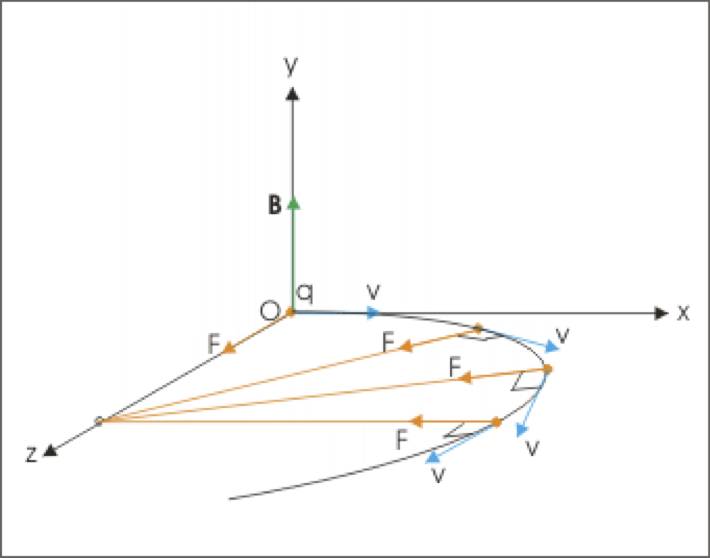
\includegraphics[width=0.45\textwidth]{giro1.png}}
  \hspace{0.3cm}
  \subfloat[]{\label{fig:giro2}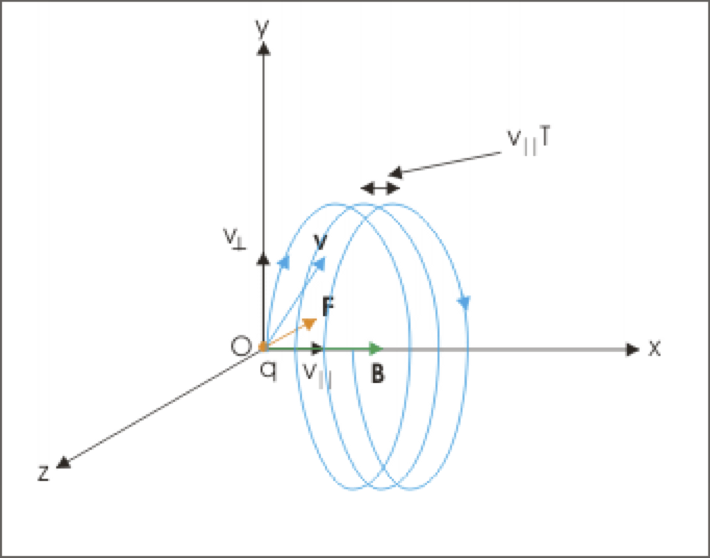
\includegraphics[width=0.45\textwidth]{giro2.png}}
  \caption{Esquematizaci\'on de la direcci\'on de la fuerza de Lorentz magn\'etica que se aplica sobre una part\'icula cargada en movimiento. (a) Un campo magn\'etico dirigido en la direcci\'on de $y$ y una part\'icula con carga $q$ que inicialmente tiene una velocidad $\vec{\text{v}}$ dirigida en direcci\'on $x$. El movimiento de esta part\'icula se es una circunferencia confinada en el plano $xz$. (b) Una trayectoria helicoidal se puede dar solamente en el caso en el que la fuerza neta que actua sobre la part\'icula cargada tenga una componente en la direcci\'on del campo magn\'etico como en el plano perpendicular a \'el. Imagenes tomadas de Singh, S. Motion of a charged particle in magnetic field, Connexions Web site. http://cnx.org/content/m31345/1.9/, Marzo 24, 2012.}
  \label{fig:helicoide}
\end{figure}

Para analizar en detalle la emisi\'on electromagn\'etica producto de este movimiento helicoidal de una part\'icula cargada es necesario considerar la forma en que los campos el\'ectricos y magn\'eticos se ven afectados y, por ende, la forma en la que una se\~nal electromagn\'etica es transmitida. Para desarrollar este an\'alisis se necesita apelar a los conocidos potenciales retardados de {\it Li\'enard-Wiechert} en donde despu\'es de algunas consideraciones f\'isicas y un extensivo desarrollo algebraico (ver por ejemplo \citep[]{jackson1975} o \citep[]{Schwartz1987}) se llega a una expresi\'on que da cuenta de la potencia energ\'etica radiada por unidad de \'angulo s\'olido como:

\begin{align}\label{eq:pot}
\frac{dP}{d\Omega}=\frac{e^2a^2}{4\pi c^3}\frac{(1-\beta \cos\theta')^2-(1-\beta^2)\sin^2\theta'\cos^2\varphi}{(1-\beta\cos\theta')^5}
\end{align}

\noindent donde nuevamente $e$ es la carga de cada part\'icula, $a$ es aceleraci\'on centr\'ipeta, $c$ es la velocidad de porpagaci\'on de una onda electromagn\'etica en el medio, $\beta$ es la velocidad de la part\'icula (en unidades de $c$), $\theta'$ es el \'angulo de polar (diferente al \'angulo de cabeceo descrito anteriormente) y $\varphi$ es el \'angulo axial. La potencia total radiada se encuentra al integrar la relaci\'on (\ref{eq:pot}) en el \'angulo s\'olido \citep[]{Schwartz1987}:

\begin{align}\label{P4pi}
P=\int_{4\pi} \frac{dP}{d\Omega}\,d\Omega=\frac{2e^2a^2}{3c^3}\frac{1}{(1-\beta^2)^2}=\frac{2e^2a^2}{3c^3}\gamma^4.
\end{align}

Si se considera que la part\'icula cargada est\'a inmersa en un campo magn\'etico predominantemente unidireccional ser\'a la fuerza de Lorentz la asociada a la aceleraci\'on centr\'ipeta que gobierna el movimiento circular en el helicoide

\begin{align}
F=\gamma ma=\frac{e\text{v}B\sin\theta}{c}
\end{align}

\noindent de donde se despeja $a$ como

\begin{align}\label{avB}
a=\frac{e\text{v}B\sin\theta}{\gamma mc},
\end{align}

\noindent siendo $m$ la masa de la part\'icula en su sistema {\it pr\'opio} de referencia. Llevando (\ref{avB}) en (\ref{P4pi}) tenemos:

\begin{align}
P=\frac{2e^2\gamma^4}{3c^3}\frac{e^2\beta^2B^2\sin^2\theta}{\gamma^2m^2}=\frac{e^4}{mc^2}\frac{2}{3}\frac{B^2\gamma^2\beta^2(1-\cos^2\theta)}{mc},
\end{align}

\noindent que resulta ser la expresi\'on que aparece en la tabla \ref{procesos} que da cuenta de la perdida de energ\'ia v\'ia radiaci\'on de sincrotron midiendo la carga en unidades de la carga del electr\'on y la energ\'ia medida en unidades de la energ\'ia en reposo del electr\'on $mc^2$. Todos estos procesos involucrados en el choque de un plasma son considerados en este trabajo pues nuestra finalidad es tratar de dar una explicaci\'on razonable de la forma en la que la fuente sismica es generada en aquellos eventos ac\'usticos observados asociados a eventos de fulguraci\'on solar y que es la materia que hoy en d\'ia conforma la rama conocida como la {\it Heliosismolog\'ia local} que ser\'a el tema que trataremos a continuaci\'on.


\subsection*{Reflexi\'on magn\'etica}
\addcontentsline{toc}{subsection}{Reflexi\'on magn\'etica}


Seg\'un los modelos actuales, la distribuci\'on de l\'ineas de campo magn\'etico a lo largo de un bucle solar es algo como lo que se representa en la figura \ref{fig:bucle}, en donde la densidad de l\'ineas aumenta progresivamente de forma sim\'etrica a partir de la cima del bucle y a medida que se avanza hacia las bases de \'el. Si se supone que la configuraci\'on de campo magn\'etico es tal que no varia con el tiempo, entonces cualquier part\'icula cargada el\'ectricamente que se mueva en una trayectoria helicoidal desde la cima del bucle en direcci\'on hacia alguna de sus bases sufrir\'a una reflex\'ion en un punto debido justamente al aumento progresivo de la densidad de l\'ineas de campo magn\'etico. Para entender esto desde un punto de vista formal, debemos empezar por recordar el concepto de invarianza adiab\'atica de algunas cantidades asociadas a un sistema f\'isico din\'amico.\\

El teorema de la invarianza adiab\'atica implica que las integrales de acci\'on no var\'ian cuando se produce un cambio que es lo suficientemente lento comparado con los periodos de movimiento del sistema f\'isico y adem\'as dichos cambios no set\'an relacionados de forma alguna con los periodos. Sea $q_i$ el conjunto de coordenadas generalizadas del sistema donde $i$ indexa a cada una de estas variables, y $p_i$ los momentos can\'onicos conjugados generalizados de cada una de las variables respectivamente. Toda coordenada peri\'odica define una integral de acci\'on

\begin{align}
J_i=\oint p_i\,dq_i.
\end{align}

El movimiento transversal de una part\'acula cargada en un campo magn\'etico est\'atico es un movimiento peri\'odio, de manera que se puede definir la integral de acci\'on siguiente

\begin{align}\label{eq:j}
\vec{J}=\oint \vec{P}_\perp\cdot d\vec{l},
\end{align}

\noindent donde $\vec{P}_\perp$ es la componente del momentum magn\'etico que es perpendicular a las l\'ineas de campo magn\'etico en cada punto, y $d\vec{l}$ es la diferencial de longitud a lo largo del c\'irculo instant\'aneo de la part\'icula definido en su \'orbita helicoidal a lo largo de las l\'ineas de campo magn\'etico que es justamente el camino sobre el cual se eval\'ua la integral. El vector momentum $\vec{P}$ es

\begin{align} 
\vec{P}=\gamma m\vec{\text{v}}+\frac{e}{c}\vec{A},
\end{align}

\noindent de manera que reemplazando expl\'icitamente en la ecuaci\'on (\ref{eq:j}) tenemos

\begin{align}\label{eq:j1}
\vec{J}=\oint\gamma m\vec{\text{v}}_\perp\cdot d\vec{l}+\frac{e}{c}\oint\vec{A}\cdot d\vec{l}.
\end{align}

De la primera integral de la ecuaci\'on (\ref{eq:j1}) se tiene que

\begin{align}
\vec{\text{v}}\cdot d\vec{l}&=(\omega_B\,a\,\hat{\theta})\cdot(a\,d\theta\,\hat{\theta})\\
&=\omega_B\,a^2\,d\theta,
\end{align}

\noindent siendo $\vec{a}$ el radio instant\'aneo descrito por la \'orbita de la part\'icula, $\omega_B$ la frecuencia angular (conocida tambi\'en como {\it frecuencia de Larmor} definida por $\omega_B=\frac{eB}{\gamma mc}$) y $\theta$ el \'angulo barrido sobre la circunferencia. De esta manera (\ref{eq:j1}) se re-escribe como

\begin{align}
\vec{J}=\oint\gamma\, m\,\omega_B\, a^2\,d\theta+\frac{e}{c}\oint\vec{A}\cdot d\vec{l};
\end{align}

\noindent aplicamos el teorema de {\it Stokes} sobre este t\'ermino

\begin{align}
\vec{J}=\oint\gamma\,m\,\omega_B\,a^2\,d\theta-\frac{e}{c}\int_S(\vec{\nabla}\times\vec{A})\cdot\hat{n}\,da,
\end{align}

\noindent en donde $S$ es la superficie encerrada por la circunferencia instant\'anea de la trayectoria de la part\'icula, y el signo negativo del segundo t\'ermino aparece porque el vector unitario $\hat{n}$ se dirige en sentido contrario a las l\'ineas de campo magn\'etico. De esta manera,

\begin{align}
\vec{J}&=\oint\gamma\,m\,\omega_B\,a^2\,d\theta-\frac{e}{c}\int_S\vec{B}\cdot\hat{n}\,da\\\label{eq:j2}
&=2\pi\,\gamma\,m\,\omega_B\,a^2+\frac{e}{c}\,|\vec{B}|\,\pi\,a^2.
\end{align}

Reemplazando expl\'incisamente la frecuencia de Larmor en (\ref{eq:j2}), tenemos

\begin{align}
\vec{J}=\gamma\,m\,\omega_B\,\pi\,a^2=\frac{e}{c}\,\underline{(B\,\pi\,a^2)},
\end{align}

\noindent en donde el \'ultimo t\'ermino entre par\'entesis es el flujo magn\'etico que cruza a trav\'es de la \'orbita instant\'anea de la part\'icula.\\

Si suponemos invarianza adiab\'atica en este proceso, entonces $|\vec{J}|=cte$, y esto implica que $|\vec{B}|\,a^2=cte$, o lo que es lo mismo, que $\frac{p_\perp^2}{B}=cte$ o $\frac{\gamma e\omega_B a^2}{2c}=cte$; todas estas conocidas como cantidades que son invariantes adiab\'aticas. Ahora bien, el cambio de energ\'ia en el tiempo de la part\'icula es

\begin{align}
\frac{dE}{dt}=\vec{\text{v}}\cdot\frac{d\vec{p}}{dt},
\end{align}

\noindent mientras que la fuerza de {\it Lorentz} viene dada por

\begin{align}
\frac{d\vec{p}}{dt}=e\vec{E}+\frac{e}{c}\vec{\text{v}}\times\vec{B}+m\vec{g}.
\end{align}

Si en sistema f\'isico considerado se tiene una configuraci\'on de campo magn\'etico tal que no cambia con el tiempo, entonces

\begin{align}
\frac{d\vec{p}}{dt}\cdot\vec{\text{v}}=0,
\end{align}

\noindent de donde se deduce que $|\vec{\text{v}}|$ debe ser constante. En el caso particular de un bucle solar en el que densidad de l\'ineas de campo magn\'etico aumenta en direcci\'on hacia las capas m\'as profundas de la atm\'osfera solar, y en donde las part\'iculas cargadas el\'ectricamente viajan a trav\'es de las l\'ineas de campo describiendo \'orbitas helicoidales, la velocidad de dichas part\'iculas se puede descomponer como 

\begin{align}
\text{v}^2=\text{v}_\parallel^2+\text{v}_\perp^2
\end{align}

De esta manera, a una distancia $s_0$ a lo largo del bucle, en donde la magnitud del campo magn\'etico es $B_0$, la magnitud de la velocidad de la part\'icula ser\'a $\text{v}_0$, y se expresar\'a como $\text{v}_0^2=\text{v}_{\parallel 0}^2+\text{v}_{\perp 0}^2$. Este punto tambi\'en debe obedecer la invariabilidad adiab\'atica expresada mediante $\frac{\text{v}_{\perp 0}^2}{B_0}=cte$. Si esta constante toma el mismo valor para todo el punto sobre le bucle solar, se debe cumplir que 

\begin{align}\label{eq:adiab}
\frac{\text{v}^2_{\perp}}{B}=\frac{\text{v}_{\perp 0}^2}{B_0},
\end{align}

\noindent donde $\text{v}$ y $B$ son la velocidad de la part\'icula y la magnitud del campo magn\'etico para un punto arbitrario sobre le bucle solar. De la ecuaci\'on (\ref{eq:adiab}) se tiene

\begin{align}
\frac{\text{v}^2\sin^2\alpha}{B}=\frac{\text{v}^2_0\sin^2\alpha_0}{B_0}\\\nonumber
\sin^2\alpha=\frac{B}{B_0}\sin^2\alpha_0,
\end{align}

\noindent siendo $\alpha$ el \'angulo de inclinaci\'on entre el vector velocidad instant\'anea de una part\'acula cargada que viaja a lo largo del bucle y el vector campo magn\'etico del lugar donde se encuentra dicha part\'icula. 


En el case particular en el que $\sin^2\alpha$, $\text{v}_\perp^2=\text{v}^2$ y $\text{v}^2_\parallel=0$. Es justamente cuando se alcanza esta condici\'on que la part\'icula cargada se devuelve en su trayectoria, o sea cuando el \'angulo de inclinaci\'on es un m\'ultiplo entero de $\pi/2$.


\newpage

\section*{Simulaci\'on}
\addcontentsline{toc}{section}{Simulaci\'on}

\subsection*{Soluci\'on num\'erica de la Ecuaci\'on de Fokker-Planck dependiente del tiempo}
\addcontentsline{toc}{subsection}{Soluci\'on num\'erica de la Ecuaci\'on de Fokker-Planck dependiente del tiempo}

Con lo que se ha mostrado hasta el momento se tiene ya una idea clara de la importancia que tienen los procesos de aceleraci\'on de part\'iculas cargadas a trav\'es de un plasma magnetizado en el estudio de la astrof\'isica de {\it altas energ\'ias}\footnote{ En el contexto de este trabajo cuando nos referimos a {\it altas energ\'ias} queremos dar cuenta de aquellas energ\'ias de un conjunto de part\'iculas aceleradas asociadas a procesos no t\'ermicos. Para la inyecci\'on de un haz de part\'iculas en un bucle coronal con condiciones f\'isicas t\'ipicas (una longitud del bucle de $\sim 1.2\times10^9\,\textrm{cm}$, una magnitud de campo magn\'etico de $\sim10^2$ o $\sim 10^3$ gauss y una densidad de n\'umero que oscila entre $\sim 10^9$ y $\sim10^{14}\,\textrm{cm}^{-3}$ ) consideramos un rango que puede ir desde los $\sim10\,\textrm{keV}$ hasta $\sim 1\,\textrm{MeV}$, dependiendo de si las part\'iculas en cuesti\'on son electrones o protones.}. Adem\'as, se mostr\'o que un m\'etodo usado para la decripci\'on din\'amica de este tipo de procesos se puede trabajar mediante el uso y la soluci\'on de la ecuaci\'on de {\it Fokker-Planck} dependiente del tiempo. Este formalismo es muy general, y no se restringe \'unicamente al estudio de eventos asociados a fulguraciones solares; otros trabajos han desarrollado an\'alisis similares en la investigaci\'on de discos de acreci\'on asociados a un agujero negro, estallidos en radio, estallidos en rayos gamma, magnet\'osferas planetarias, atm\'osferas de objetos astrof\'isicos compactos, etc (ver por ejemplo \cite{cohn1978} y \cite{becker2006}). Ahora bien, dependiendo de los par\'ametros f\'isicos del plasma como la densidad de n\'umero, la magnitud del campo magn\'etico, y la energ\'ia de las part\'iculas inyectadas, algunos procesos fenomenol\'ogicos van a ser m\'as relevantes que otros. Con el \'animo de simplificar suficientemente el problema de manera tal que sea posible llevar a cabo la simulaci\'on, pero teniendo cuidado de no perder demasiada informaci\'on f\'isica importante en la din\'amica del proceso de aceleraci\'on, presentamos aqu\'i una ecuaci\'on de {\it Fokker-Planck} que \cite{hamilton1990} han propuesto con anterioridad para llevar a cabo un estudio razonable de la aceleraci\'on de part\'iculas en un evento de fulguraci\'on solar.\\

La ecuaci\'on de {\it Fokker-Planck} es un formalismo que describe la evoluci\'on temporal de una funci\'on de densidad de probabilidad que generalmente depende de ciertas cantidades f\'isicas reales del conjunto de part\'iculas de inter\'es. Para desarrollar este tipo de an\'alisis de debe conocer con claridad las variables m\'as adecuadas para abordar este tratamiento. Inicialmente se desear\'ia que dicha funci\'on dependiera de alguna variable espacial. En el caso de los bucles solares la trayectoria que siguen las part\'iculas es gobernada principalmente por la geometr\'ia del campo magn\'etico en un movimiento que, como ya se mencion\'o anteriormente, se conoce como giro-movimiento. El giro-radio, definido como el radio de la circunferencia instant\'anea de la trayectoria de cada una de las part\'iculas cargadas en su movimiento a lo largo de un campo magn\'etico localmente uniforme, que en el caso no-relativista\footnote{En el caso de los electrones, un tratamiento no-relativista de la componente no-t\'ermica de la energ\'ia se limita a trabajar en la banda entre los 10 keV y los 100 keV que corresponde a velocidades entre los 0.02c y 0.2c  respectivamente. Con este acotamiento en las energ\'ias garantizamos una diferencia no mayor al 3\% entre el an\'alisis que aqu\'i presentamos y un tratamiento que incluya los t\'erminos relativistas. Este c\'alculo del error se hace usando la expresi\'on para la energ\'ia cin\'etica relativista de una part\'icula $E_c=m_0c^2\left[\frac{1}{\sqrt{1-\text{v}^2/c^2}}-1\right]$, expandiendo esta expresi\'on usando el teorema del binomio $(a+x)^n=a^n+na^{n-1}x+\frac{n(n-1)}{2!}a^{n-2}x^2+...$ y comparando el valor obtenido con el calculado mediante la expesi\'on cl\'asica para la energ\'ia cin\'etica $E_c=\frac{1}{2}m_e\text{v}^2$.} es igual a

\begin{align}\label{giroradio}
r_g=\frac{m_e\text{v}_\perp}{q_eB},
\end{align}

\noindent en donde $m_e$ es la masa en reposo de un electr\'on, $B$ es la magnitud del campo magn\'etico local, $\text{v}_\perp$ es la velocidad tangencial a la \'orbita de giro instant\'anea de cada part\'icula y perpendicular a la direcci\'on de $\vec{B}$, y $q_e$ es la carga el\'ectrica de cada electr\'on. Reemplazando en la ecuaci\'on (\ref{giroradio}) los valores t\'ipicos de cada cantidad para una fulguraci\'on encontramos

\begin{align}\nonumber
r_{\text{g-fulguraci\'on}}\simeq\frac{9.11\times 10^{-31}\,\text{kg}\quad6\times 10^7\,\text{m s}^{-1}}{1.6\times 10^{-19}\,\text{C}\quad 10^{-1}\,\text{kg C}^{-1}\,\text{s}^{-1}}\simeq 3.4\times 10 ^{-3}\,\textrm{m},
\end{align}

\noindent de forma que el radio de giro resulta ser unos 10 \'ordenes de magnitud menor que la longitud t\'ipica de un bucle solar y por lo tanto se puede despreciar el movimiento helicoidal de manera que espacialmente cada part\'icula solo dependa de su posici\'on a lo largo del bucle, la cual  denotaremos como {\bf s} de aqu\'i en adelante.\\

La funci\'on de distribuci\'on en el espacio de momentum puede ser especificada por dos componentes del momentum. \cite{hamilton1990} mostraron que dos cantidades que se pueden usar para este fin son la {\it energ\'ia} ({\bf E}) y el coseno del \'angulo de inclinaci\'on ($\boldsymbol{\mu}$). De esta manera la funci\'on de distribuci\'on depende de cuatro variables $W=W(E,\mu,s,t)$, siendo $t$ el tiempo. Esta funci\'on de distribuci\'on obedece la ecuaci\'on de {\it Fokker-Planck} mostrada en (\ref{fph}), el problema se reduce entonces a resolver dicha ecuaci\'on. Aunque existe un par de soluciones anal\'iticas de esta ecuaci\'on bajo restricciones fuertes, en general la forma de resolverla debe ser mediante el uso de un m\'etodo num\'erico. Existen varias t\'ecnicas disponibles para atacar el problema num\'ericamente. Siguiendo a \cite{hamilton1990}, nosotros usamos la t\'ecnica de {\it diferencias finitas} junto con la de {\it operador de divisi\'on} (en ingl\'es {\it time operator splitting}).

\subsubsection*{M\'etodo de diferencias finitas}
\addcontentsline{toc}{subsubsection}{M\'etodo de diferencias finitas}

El m\'etodo consiste en solucionar una determinada ecuaci\'on diferencial parcial que evoluciona linealmente en el tiempo haciendo que esta sea igual a la suma de ciertos operadores diferentes $\hat{\mathcal{O}}_i$ que act\'uan sobre la funci\'on evolutiva y dependen de la ecuaci\'on diferencial en particular que se quiere solucionar, como se muestra:

\begin{align}
\frac{\partial}{\partial t} W(\mathbf{x},t)=\sum_{i=0}^{k}\hat{\mathcal{O}}_i[W(\mathbf{x},t)],
\end{align}

\noindent en donde $\mathbf{x}$ es el vector en el espacio de fase (aqu\'i $\mathbf{x}$ representa $E$, $\mu$ y $s$), $W$ es al menos de clase $C^3$ y los $\hat{\mathcal{O}}_i$ son operadores diferenciales ($i\geq1$) o multiplicativos ($i=0$). De acuerdo con el m\'etodo del operador de divisi\'on, uno puede expresar la funci\'on $W(\mathbf{x},t+\Delta t)$ como una aplicaci\'on sucesiva de operadores diferencias sobre la funci\'on $W(\mathbf{x},t)$ de modo tal que dicha aplicaci\'on sucesiva se aproxime al operador diferencial $\hat{\mathcal{O}}_i$ y hace que la funci\'on $W$ avance en un paso de tiempo $\Delta t$. 

\begin{align}
W(\mathbf{x},t+\Delta t)=\Phi_k(\Phi_{k-1}[\ldots\Phi_2(\Phi_1[W(\mathbf{x},t),\Delta t],\Delta t)\ldots,\Delta t],\Delta t),
\end{align}

De esta manera se hace la aproximaci\'on entre la ecuaci\'on diferencial real y una sucesi\'on de ecuaciones de diferenciales finitas que dependen del orden de las derivadas en consideraci\'on, de modo tal que si:

\begin{align}\nonumber
&\text{si}\quad i =1,\qquad \hat{\mathcal{O}}_1[W(\mathbf{x},t)]\rightarrow W(\mathbf{x},t+\Delta t)=\Phi_1(W,\Delta t),\\
&\text{si}\quad i=2,\qquad \hat{\mathcal{O}}_2[W(\mathbf{x},t)]\rightarrow W(\mathbf{x},t+\Delta t)=\Phi_2[\Phi_1(W,\Delta t)],
\end{align}

\noindent etc. Con esta descripci\'on del m\'etodo ya es posible entrar a analizar en detalle cada t\'ermino en la ecuaci\'on (\ref{fph}). Una forma general operacional de la ecuaci\'on (\ref{fph}) es 

\begin{align}\label{eq:form}
-\frac{\partial W}{\partial t}=g(\mathbf{x},t)+\sum_{j=1}^3f_j(\mathbf{x})\frac{\partial}{\partial x_j}(V_j(\mathbf{x})W(\mathbf{x},t))+q(\mathbf{x})\frac{\partial}{\partial\mu}\left(h(\mu)\frac{\partial W(\mathbf{x},t)}{\partial \mu}\right)
\end{align}

\noindent en donde $j=1,2,3$ representa a las variables $E,\mu,s$. Para continuar con el an\'alisis consideraremos m\'as adelante los t\'erminos de cada una de las variables en la ecuaci\'on (\ref{fph}). En este m\'etodo num\'erico usualmente se toman las variaciones con respecto a $s,E,\mu$, en forma independiente, como si la variaci\'on temporal de la funci\'on de distribuci\'on $W$ con respecto al tiempo, $-\partial W/\partial t$, variase en forma independiente con respecto a las tres variables citadas anteriormente, de modo tal que consideraremos cada una de estas variaciones como una ecuaci\'on diferencial m\'as sencilla, la cual se resuelve, y al final la suma de las tres contribuciones se considerar\'a como la variaci\'on total de $W$ con respecto del tiempo. Para facilitar nuestra nomenclatura cada una de las variaciones de $W$ con respecto del tiempo, encontradas de la forma citada, las llamaremos $W_s$, $W_E$, $W_\mu$, sin que ello denote una naturaleza vectorial de $W$.




%Una observaci\'on m\'as detallada de la ecuaci\'on (\ref{fph}) permite ver que para la posici\'on y la energ\'ia el \'ultimo t\'ermino de (\ref{eq:form}) no aparece expl\'icitamente, y la forma funcional de la dependencia de la funci\'on de distribuci\'on con respecto a cada una de estas dos variables se puede reducir a 

%\begin{align}\label{eq:fpg}
%\frac{\partial}{\partial t}W(\mathbf{x},t)=-\frac{\partial}{\partial x_j}[V(\mathbf{x})W(\mathbf{x},t)],
%\end{align}

%\noindent donde $V(\mathbf{x})$ es una funci\'on determinada del vector $\mathbf{x}$ del espacio de fase, mientras que $x_j$ representa a cada una de las variables $E$ y  $s$. De esta manera se observa f\'acilmente que la ecuaci\'on (\ref{eq:fpg}) es una ecuaci\'on de transporte en la que la funci\'on de distribuci\'on de los electrones $W(\mathbf{x},t)$ se mueve con una tasa $V(\mathbf{x})$ definida sobre el espacio de fase en energ\'ia y posici\'on. 

\subsubsection*{Dependencia con la posici\'on}

N\'otese que en este t\'ermino la rapidez v es independiente de la posici\'on a lo largo del bucle $s$ de manera que el tratamiento se simplifica. La ecuaci\'on a considerar es 

\begin{align}
\frac{\partial W_s}{\partial t}=-\mu \text{v}\frac{\partial W}{\partial s},
\end{align}

A este tipo de ecuaci\'on se le conoce con el nombre de {\it ecuaci\'on de transporte mon\'otono}. Para este tipo de ecuaciones el mejor m\'etodo que puede ser usado para solucionarla es justamente el de diferencias finitas \citep{hawley1984}. La funci\'on de distribuci\'on $W_s(s,t+\Delta t)$ se expresa como

\begin{align}
&W_s(s,t+\Delta t)=\\\nonumber
&\begin{cases}
W_s(s,t)-\mu\text{v}\frac{\Delta t}{\Delta s}[W_s(s,t)-W_s(s-\Delta s,t)] - \mu\text{v}\frac{\Delta t}{\Delta s}(1-\mu\text{v}\frac{\Delta t}{\Delta s})[\Delta W_s(s,t)-\Delta W_s(s-\Delta s,t)],\quad \text{para}\quad \mu\text{v}\frac{\Delta t}{\Delta s}>0,\\
W_s(s,t)-\mu\text{v}\frac{\Delta t}{\Delta s}[W_s(s+\Delta s,t)-W_s(s,t)] - \mu\text{v}\frac{\Delta t}{\Delta s}(1-\mu\text{v}\frac{\Delta t}{\Delta s})[\Delta W_s(s+\Delta s,t)-\Delta W_s(s,t)],\quad \text{para}\quad \mu\text{v}\frac{\Delta t}{\Delta s}<0;
\end{cases}
\end{align}

\noindent en donde $\Delta s$ es el tama\~no del paso en la divisi\'on que se establezca a lo largo de la longitud del bucle y 

\begin{align}
\Delta W_s(s,t)=
\begin{cases}
\frac{[W_s(s,t)-W(s-\Delta s,t)][W_s(s+\Delta s,t)-W_s(s,t)]}{[W_s(s+\Delta s,t)-W_s(s-\Delta s,t)]},\quad\text{para}\quad[W_s(s,t)-W_s(s-\Delta s,t)][W_s(s+\Delta s,t)-W_s(s,t)]>0,\\
0,\quad\text{para el resto.}
\end{cases}
\end{align}

\subsubsection*{Dependencia con la energ\'ia}

Para este t\'ermino la velocidad de transporte $V(\mathbf{x},t)$ en la ecuaci\'on (\ref{eq:fph}) depende expl\'icitamente de la energ\'ia, de manera que para proponer una soluci\'on se define la funci\'on $\mathcal{W}_E=VW_E$ y $d\mathcal{E}=V\,dE$; de esta manera el problema se reduce al que ya se resolvi\'o arriba y se puede llevar a cabo usando el mismo m\'etodo. En este caso se aplica el algoritmo descrito por \cite{centrella1984}. As\'i

\begin{align}
W_E(E',t+\Delta t)=W_E(E',t)-\frac{\Delta t}{\Delta E}[V_E(E'+\Delta E/2)W(E'+\Delta E/2,t)-V_E(E'-\Delta E/2)W(E'-\Delta E/2,t)].
\end{align}

F\'isicamente, $V_E(E'+\Delta E/2)W(E'-\Delta E/2,t)$ y $V_E(E'+\Delta E/2)W(E'-\Delta E/2,t)$ son el flujo que sale y que entra respectivamente a la celda num\'erica centrada en el valor de energ\'ia particular $E'$ (en el caso en el que $V_E<0$ entonces los flujos ser\'an negativos). El valor de $W_E(E'-\Delta E/2,t)$ est\'a dado por 

\begin{align}\nonumber
&\text{si}\,V_E>0:W_E(E'-\Delta E/2,t)=
\begin{cases}
\min[W(E'-\Delta E),\max\lbrace\mathcal{W}(E',t),\overline{W}(E',t)\rbrace],\quad W(E',t)\leq W(E'-\Delta E,t)\\
\max[W(E'-\Delta E),\min\lbrace\mathcal{W}(E',t),\overline{W}(E',t)\rbrace],\quad W(E',t)> W(E'-\Delta E,t)
\end{cases},\\
&\text{si}\,V_E<0:W_E(E'-\Delta E/2,t)=
\begin{cases}
\max[W(E'),\min\lbrace\mathcal{W}(E',t),\overline{W}(E',t)\rbrace],\quad W(E',t)\leq W(E'-\Delta E,t)\\
\min[W(E'),\max\lbrace\mathcal{W}(E',t),\overline{W}(E',t)\rbrace],\quad W(E',t)> W(E'-\Delta E,t)
\end{cases},
\end{align}

\noindent con $\overline{W}(E',t)=\dfrac{W(E',t)+W(E'-\Delta E)}{2}$, y

\begin{align}
\mathcal{W}(E',t)=
\begin{cases}
\frac{3}{2}W(E'-\Delta E,t)-\frac{1}{2}W(E'-2\Delta E,t),\quad\text{para}\,V_E>0\\
\frac{3}{2}W(E',t)-\frac{1}{2}W(E'+\Delta E,t),\quad\text{para}\,V_E<0
\end{cases}.
\end{align}

\subsubsection*{Dependencia con el \'angulo de inclinaci\'on (t\'ermino difusivo)}

El t\'ermino de dispersi\'on por colisi\'on Coulombiana en la ecuaci\'on (\ref{fph}) hace que aparezca un t\'ermino difusivo en la dependencia con el \'angulo de inclinaci\'on de la ecuaci\'on de {\it Fokker-Planck} adem\'as del t\'ermino convectivo, como lo podemos apreciar en la siguiente expresi\'on: 

\begin{align}
\frac{\partial}{\partial t }W_\mu(\mathbf{x},t)=\text{v}\frac{d\,\ln\,B}{ds}\frac{\partial}{\partial\mu}\left(\frac{(1-\mu^2)}{2}W\right)+\frac{c^4}{\lambda_0\text{v}^3\gamma^2}\frac{\partial}{\partial \mu}\left[(1-\mu^2)\frac{\partial W}{\partial \mu}\right].
\end{align}

Esta ecuaci\'on tiene la forma funcional:

\begin{align}
\frac{\partial}{\partial t }W_\mu=B(\mu)\frac{\partial W_\mu}{\partial \mu}+C(\mu)\frac{\partial^2W_\mu}{\partial \mu^2},
\end{align}

\noindent la cual puede ser solucionada num\'ericamente usando el m\'etodo de {\it Crank-Nicholson} \citep{smith1985}. Expl\'icitamente,

\begin{align}\nonumber
\frac{W_\mu(\mu,t+\Delta t)-W_\mu(\mu,t)}{\Delta t}=
\frac{B_\mu}{2}&\left[\frac{W_\mu(\mu+\Delta\mu,t)-W_\mu(\mu-\Delta\mu,t)}{2\Delta\mu}+\frac{W_\mu(\mu+\Delta\mu,t+\Delta t)-W_\mu(\mu-\Delta\mu,t+\Delta t)}{2\,\Delta\mu}\right]\\\nonumber
+\frac{C_\mu}{2\Delta\mu}&\left[\left(\frac{W_\mu(\mu+\Delta\mu,t)-W_\mu(\mu,t)}{\Delta\mu}-\frac{W_\mu(\mu,t)-W_\mu(\mu-\Delta\mu,t)}{\Delta\mu}\right)\right. \\
&\left. +\left(\frac{W_\mu(\mu+\Delta\mu,t+\Delta t)-W_\mu(\mu,t+\Delta t)}{\Delta\mu}-\frac{W_\mu(\mu,t+\Delta t)-W_\mu(\mu-\Delta\mu,t+\Delta t)}{\Delta\mu}\right)\right].
\end{align}


\subsection*{C\'odigo num\'erico}
\addcontentsline{toc}{subsection}{C\'odigo num\'erico}

Teniendo en cuenta los algoritmos expuestos anteriormente para la soluci\'on num\'erica de la ecuaci\'on de {\it Fokker-Planck} dependiente del tiempo, \citeauthor{hamilton1990} desarrollaron un conjunto de c\'odigos en 1997 escritos en FORTRAN que solucionan la ecuaci\'on bajo las condiciones f\'isicas t\'ipicas (seg\'un la literatura cient\'ifica) de la aceleraci\'on de electrones en una fulguraci\'on solar. A\~nos m\'as tarde \cite{Holman2001} desarrollaron mejoras en velocidad y eficiencia de c\'omputo de este conjunto de programas e implementaron unos c\'odigos escritos en lenguaje IDL (de sus siglas en ingl\'es {\it Interactive Data Language}) para facilitar la visualizaci\'on de los resultados. Todos estos programas han sido publicados en la internet en la p\'agina \url{http://hesperia.gsfc.nasa.gov/hessi/modelware.htm} (fkrplk.zip)\footnote{Desarrollos recientes plantean otro tipo de c\'odigos para resolver esta misma ecuaci\'on. Ver por ejemplo \url{http://code.google.com/p/fokker-planck-code/downloads/list}.}; tambi\'en es posible encontrar all\'i la documentaci\'on necesaria para entender la forma general en que funcionan los c\'odigos, la forma en la que pueden ser modificados para incluir otras fenomenolog\'ias aparte de las que est\'an incluidas como lo son, emisi\'on {\it Bremsstrahlung} en rayos-X y radiaci\'on girosincrotr\'on), y la manera en la que deben ser corridos para obtener los resultados esperados \citep{Holman2001}. Este conjunto de programas consta de diez c\'odigos escritos en FORTRAN 90 que contienen todos los algoritmos necesarios para resolver la ecuaci\'on de {\it Fokker-Planck}, adem\'as de la geometr\'ia, condiciones de frontera y condiciones iniciales de jet de part\'iculas incidentes. Adem\'as contiene el programa en IDL que grafica los resultados f\'acilmente.\\

Recientemente y de manera simult\'anea al desarrollo de esta tesis {\it Paulo Simoes} ha traducido estos c\'odigos a C++ y ha introducido una manera sencilla de trabajar con diferentes tipos de funciones de inyecci\'on del conjunto incidente de part\'iculas, la funci\'on que describe la densidad del plasma ambiental, y la forma en la que el campo magn\'etico se distribuye a lo largo del bucle solar. Adem\'as, introduce en los c\'odigos el manejo de archivos binarios como archivos de salida para que sea m\'as sencilla su visualizaci\'on usando lenguajes como IDL. Inicialmente trabajamos con base en los c\'odigos desarrollados por \cite{Holman2001}, y luego trabajamos en una colaboraci\'on con el Dr. {\it Paulo Simoes} quien actualmente es investigador posdoc en la {\it School of Physics and Astronomy} de la Universidad de Glasgow (UK), para aprovechar las ventajas ya descritas de este nuevo conjunto de programas.\\

\subsubsection*{Consideraciones iniciales de la simulaci\'on}
\addcontentsline{toc}{subsubsection}{Consideraciones iniciales de la simulaci\'on}

Para abordar el problema se debe establecer qu\'e tipo de condiciones iniciales se exigen sobre las condiciones f\'isicas y geom\'etricas de la funci\'on de distribuci\'on en cada una de las variables que la gobiernan para el conjunto completo de part\'iculas inyectadas. En lo que se refiere a la dependencia energ\'etica de la funci\'on de distribuci\'on, apelamos a los trabajos desarrollados por \cite{lu1988} en los que mostraron que la intensidad de flujo asociada a las fases impulsiva y de decaimiento de una fulguraci\'on solar tiene una dependencia expresada mediante

\begin{align}
I(E,t)=I_{E_0}(t)\left(\frac{E}{E_0}\right)^{-\gamma(t)},
\end{align}

\noindent donde $E_0$ es una energ\'ia de referencia (que usualmente se toma como 50keV) y $\gamma$ es el \'indice espectral para los fotones provenientes de la fulguraci\'on. 

\begin{wrapfigure}[25]{r}{0.46\textwidth}
\begin{center}
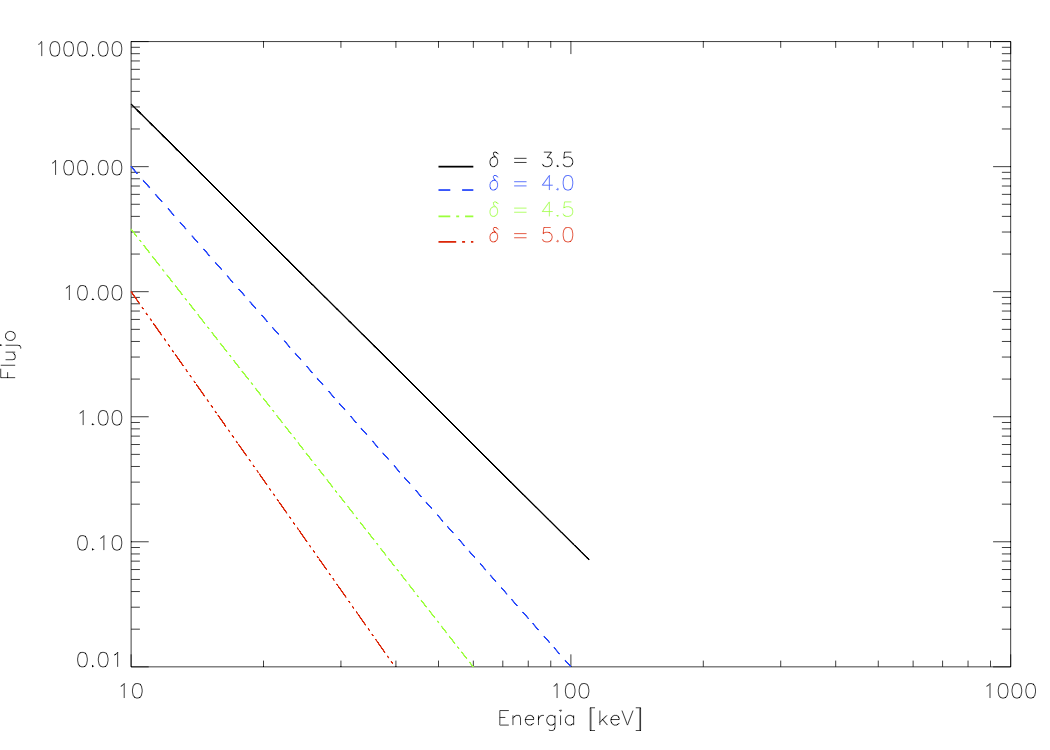
\includegraphics[width=0.39\textwidth]{delta.png}
\caption{Ejemplo de las distribuciones tipo ley de potencias usadas para ajustar la parte de emisi\'on no-t\'ermica de un espectro t\'ipico de una fulguraci\'on solar con una emisi\'on discernible en rayos-X duros. Como se ejemplifica en el cuadro \ref{table:kontar} los \'indices $\delta$ usualmente toman valores entre 3.5 y 5.0. Para la distribuci\'on energ\'etica de la distribuci\'on de densidad electr\'onica que se introduce como {\it input} en nuestra simulaci\'on usamos valores para $\delta$ en el rango que se muestra aqu\'i.}
\label{fig:delta}
\end{center}
\end{wrapfigure}

Por otro lado, si se asume que la funci\'on de distribuci\'on de densidad electr\'onica obedece tambi\'en una ley de potencias, es decir $f_{\text{electrones}}\propto E^{-\delta}$, el \'indice de la ley de potencia $\delta$ debe estar relacionado de alguna manera con el \'indice espectral $\gamma$. As\'i, dependiendo del tipo de interacci\'on entre los electrones acelerados y el plasma del ambiente circundante a la posici\'on donde la emisi\'on fot\'onica tiene lugar, esta relaci\'on toma una forma que depende esencialmente del mecanismo dominante de radiaci\'on. \cite{Tandberg-Hanssen1988} hacen una descripci\'on de este tipo de relaci\'on entre los dos \'indices a trav\'es de los dos modelos que han demostrado mayor \'exito hasta el momento en su contraste con los resultados observacionales, el llamado modelo de {\bf blanco grueso} ({\it thick target model}) y el modelo de {\bf blanco delgado} ({\it thin target model}). Seg\'un estos modelos, esta relaci\'on est\'a dada por

\begin{align}
\gamma_{thin}=\delta + 0.5\qquad\gamma_{thick}=\delta - 1.5\text{.}
\end{align}

La realidad es que el valor num\'erico de estos \'indices de deben encontrar de forma emp\'irica. Muchos trabajos en torno al mejor ajuste de los espectros observacionales de diferentes fulguraciones han sido desarrollados, obteniendo rangos de validez para estos \'indices entre $2\lesssim\delta\lesssim8$ y $3\lesssim\gamma\lesssim9$ \citep{grigis2006}. Un ejemplo de este tipo de an\'alisis observacional lo muestran \cite{kontar2002}, quienes para cuatro eventos de fulguraciones altamente energ\'eticas reportan valores de \'indice espectral de los electrones como se puede apreciar en el cuadro \ref{table:kontar}.

\begin{table}
\centering
\begin{tabular}{ l c c }\hline
Fecha & Hora (TU) & $\delta$ \\\hline
  20 Feb 2002 & 11:06:00 - 11:06:40 & 4.89 \\
  17 Mar 2002 & 19:27:30 - 19:29:10 & 4.84 \\
  31 May 2002 & 00:06:40 - 00:08:00 & 3.79 \\
  01 Jun 2002 & 03:53:10 - 03:54:30 & 4.26 \\\hline
\end{tabular}
\caption{\'Indice de la ley de potencias que obedece la distribuci\'on de densidad de electrones para cuatro fulguraciones diferentes que tuvieron lugar en 2002. El valor de cada \'indice se determin\'o usando un blanco ionizado uniforme bajo el protocolo usado por defecto por SPEX, el software especializado de RHESSI para estos menesteres \cite[]{kontar2002}.}
\label{table:kontar}
\end{table}

Teniendo en cuenta lo anterior, no estamos muy lejos de la realidad f\'isica si para el tiempo inicial imponemos que la distribuci\'on de densidad electr\'onica en funci\'on de la energ\'ia obedecer\'a una ley de potencia con \'indice $\delta=4.5$. En general, 

\begin{align}
f_{\text{electrones}}=A_e(m_ec^2)^{-\delta}
\end{align}

\noindent donde $A_e$ es una constante de ajuste al espectro seg\'un el flujo que se tenga y $m_ec^2$ es la energ\'ia total de un electr\'on t\'ipico (la suma de la energ\'ia en reposo m\'as su energ\'ia cin\'etica).\\

\begin{wrapfigure}[31]{r}{0.5\textwidth}
\begin{center}
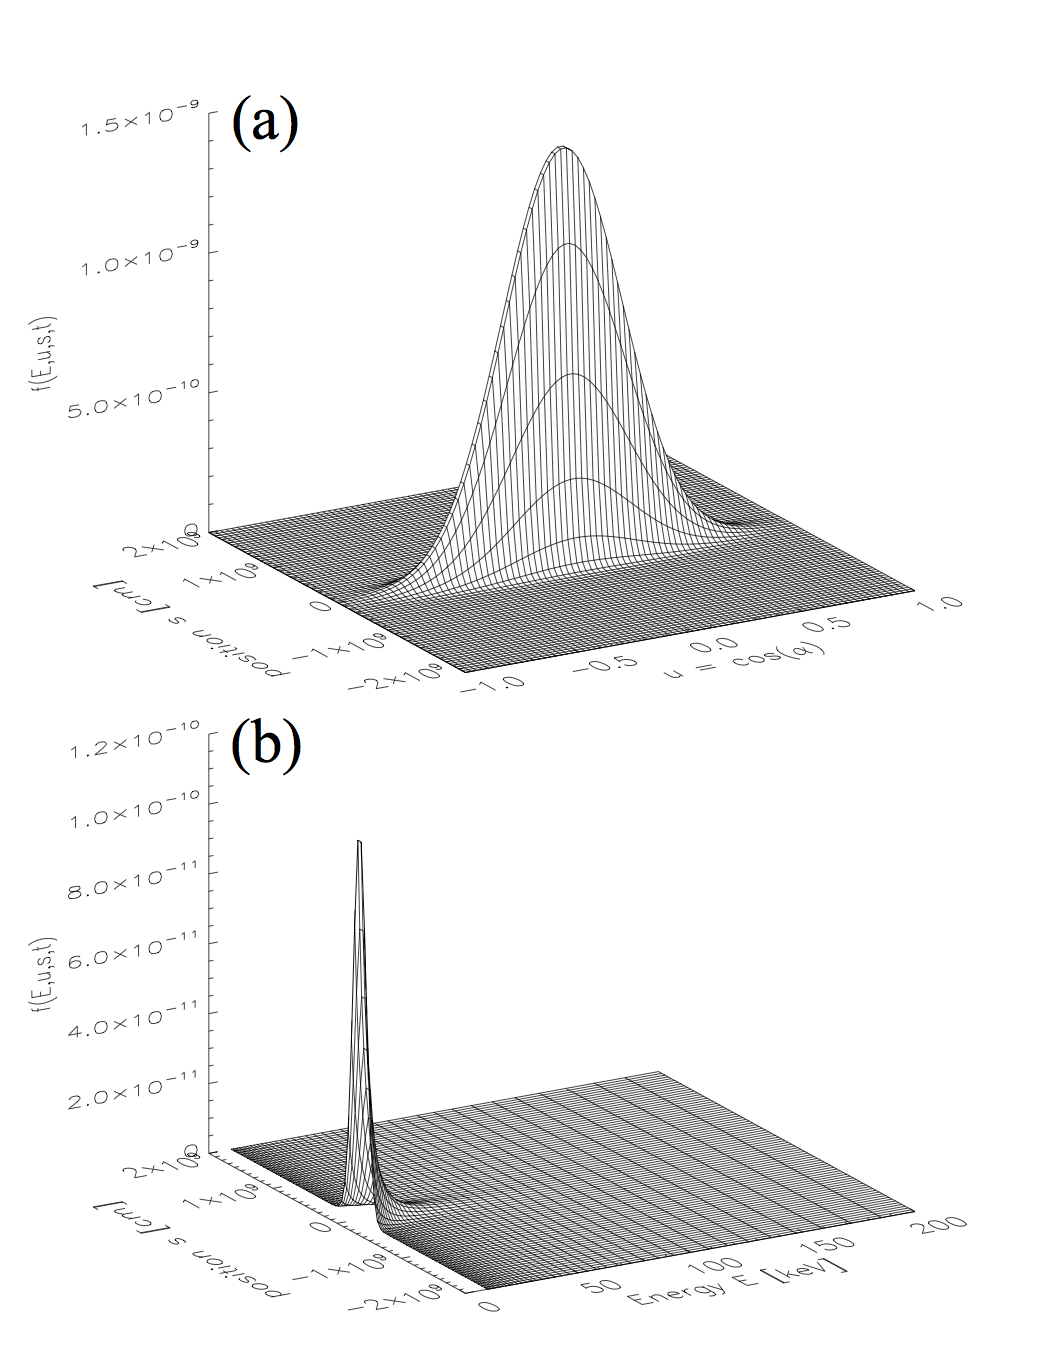
\includegraphics[width=0.5\textwidth]{input.png}
\caption{Funci\'on de entrada para la distribuci\'on de densidad de probabilidad electr\'onica. {\bf (a)} Dependencia gaussiana con la posici\'on y el \'angulo de inclinaci\'on. {\bf (b)} Dependencia con la posici\'on y la energ\'ia.}
\label{fig:input}
\end{center}
\end{wrapfigure}

Siguiendo con la discusi\'on de c\'omo debe ser la distribuci\'on inicial del programa que resuelve num\'ericamente la ecuaci\'on de {\it Fokker-Planck} en funci\'on de cada una de las variables de las que depende, ahora es el turno de discutir la distribuci\'on inicial de la densidad electr\'onica en funci\'on del \'angulo de inclinaci\'on $\alpha$, o equivalentemente del coseno de este, $\mu=\cos\alpha$. Una vez el {\it jet} de part\'iculas es inyectado en el bucle solar por la cima de este, la direcci\'on en la que inciden cada una de ellas tiene un sentido preferencial que resulta ser perpendicular a las l\'ineas de campo magn\'etico en esa localidad, es decir $\cos\alpha=0$. Este proceso de inyecci\'on est\'a acompa\~nado de varios fen\'omenos aleatorios, la distribuci\'on incidente se debe poder modelar como una distribuci\'on gaussiana con cierto valor de desviaci\'on est\'andar. As\'i, $f_\alpha = A_\alpha\exp\left[-\frac{\mu^2}{2\,d\mu^2}\right]$, siendo $A_\alpha$ una constante de normalizaci\'on o de ajuste y $d\mu$ la desviaci\'on est\'andar. Algunos trabajos se han desarrollado tratando de describir la mejor funci\'on de distribuci\'on en funci\'on del \'angulo de inclinaci\'on que mejor se acomode a los resultados observacionales y que pueda ser usada como par\'ametro de entrada en los diferentes c\'odigos num\'ericos relacionados con este fen\'omeno. Siguiendo a \cite{2000leegary} nosotros usamos para $t=0$, los valores iniciales $\mu=0$ para el coseno del \'angulo de inclinaci\'on $\alpha$ y $d\mu=0.26$ para su desviaci\'on est\'andar respectivamente.\\

Usamos tambi\'en una distribuci\'on con dependencia gaussiana en la posici\'on, esto es

\begin{align}
f_s = A_s\exp\left[-\frac{s^2}{2\,ds^2}\right],
\end{align}

\noindent con $ds=10^{8}$ cm (dos \'ordenes de magnitud menor que la longitud t\'ipica de un bucle solar), en donde $ds$ es la desviaci\'on est\'andar respectiva. De esta manera, la distribuci\'on de densidad de probabilidad en funci\'on de la posici\'on, el \'angulo de inclinaci\'on y de la posici\'on para el momento de la inyecci\'on (que usamos como par\'ametro de entrada de nuestra simulaci\'on) es algo como lo que se muestra en a figura \ref{fig:input}.\\

Es importante precisar tambi\'en la forma temporal en la que deben ser inyectadas las part\'iculas en la cima del bucle. Num\'ericamente lo m\'as sencillo es hacer que todo el conjunto de part\'iculas aparezcan en la cima s\'ubitamente para un tiempo dado (el tiempo inicial) tal y como funciona el c\'odio original desarrollado por \cite{hamilton1990}. Sin embargo, esto no es del todo cierto durante el fen\'omeno f\'isico real; en el momento de la inyecci\'on las part\'iculas arriban al bucle con cierta distribuci\'on temporal. Siguiendo a \cite{aschwanden2004}, este tiempo de inyecci\'on de las part\'iculas es m\'as importante que el tiempo en el cual se hayan acelerado las part\'iculas, previas a su incidencia sobre la cima del bucle, para determinar la escala de tiempo de emisi\'on en rayos-X duros, y lo cual es lo que nos caracteriza la din\'amica del proceso post-reconexi\'on.\\

Una vez definida la f\'isica detr\'as de la inyecci\'on del conjunto de electrones acelerados en la cima de bucle solar podemos centrarnos m\'as en los detalles t\'ecnicos relacionados con los par\'ametros iniciales que se deben suministrar al conjunto de programas que resuelve la ecuaci\'on de {\it Fokker-Planck} dependiente del tiempo que es justamente el tema que abordamos a continuaci\'on.





%Hacer gr�fica de alpha vs. t .... como son variables linealmente independientes esta dependencia da una l�nea reca creciente.

%introducir alpha=0 a ver que pasa

% Pilas con esto para las conclusiones y la variaci�n de la corrida del programa: AshwandenLa duraci\'on del pulso visto en rayos-X duros es controlada principalmente por el tiempo de inyecci\'on m\'as que la escala de tiempo de la aceleraci�n. Esto quiere decir que es vitalmente importante el tiempo de inyecci�n de las part�culas. 


\subsection*{Par\'ametros de entrada del conjunto de programas}
\addcontentsline{toc}{subsection}{Par\'ametros de entrada del conjunto de programas}


\begin{wrapfigure}[25]{l}{0.46\textwidth}
\begin{center}
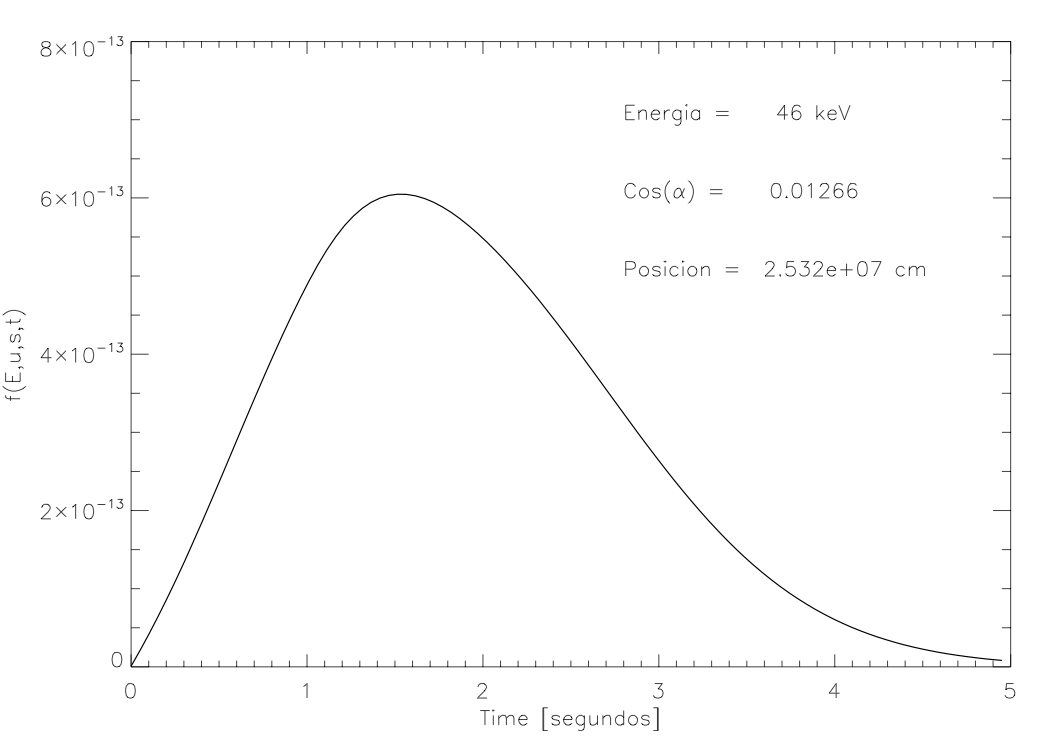
\includegraphics[width=0.44\textwidth]{image_ft.png}
\caption{Evoluci\'on temporal de la distribuci\'on de densidad de probabilidad electr\'onica usado en la simulaci\'on con una energ\'ia de 46 keV, una \'angulo de inclinaci\'on de $89.3^\circ$ y una posici\'on fija de $2.532\times10^{7}$ cm. Se ve claramente que la funci\'on de inyecci\'on de part\'iculas obedece una forma gaussiana y que la intensidad m\'axima de inyecci\'on se alcanza cerca de $\sim 1$ segundo como propone \cite{aschwanden2004}.}
\label{fig:tf}
\end{center}
\end{wrapfigure}

Definir el tama\~no de la grilla:  {\bf ned} es la cantidad de pasos en energ\'ia (por defecto usamos 40), {\bf nud} es la cantidad de pasos en el \'angulo de inclinaci\'on (por defecto usamos 80), {\bf nsd} es la cantidad de pasos en la longitud del bucle (por defecto usamos 80), {\bf ntd} es la cantidad de pasos en tiempo (por defecto usamos 100). Se definen los l\'imites en energ\'ia en keV, as\'i  {\bf emin}  define el l\'imite inferior (por defecto usamos 10), {\bf emax} define el l\'imite superior (por defecto usamos 200). Definimos los l\'imites en la posici\'on a lo largo del bucle, as\'i {\bf smin} define el l\'imite inferior en la longitud del bucle (usualmente usamos $-2\times10^9$ m) y {\bf smax} define el l\'imite superior en la longitud del bucle (usualmente usamos $2\times10^9$ m). La simulaci\'on debe contener un modelo de distribuci\'on de campo magn\'etico a lo largo del bucle, este puede ser un modelo parab\'olico dado por la expresi\'on $B(s)=B_0\times(1+s^n/LB^n)$ o un modelo exponencial dado por la ecuaci\'on $B(s) = \exp\left(\log(mr)\frac{s}{l}^n\right)$. de manera que es necesario definir la {\it raz\'on de reflejo magn\'etico} {\bf mr}$=\frac{B(s)}{B_0}$ (por defecto lo tomamos como 2); {\bf nexp} que es el exponente que va en las expresiones para el calculo del campo magn\'etico a lo largo del bucle, entre mayor sea este n\'umero mayor es el confinamiento de las part\'iculas en los pies del bucle, pero un modelo parab\'olico exige $nexp=2$. Como hay dos modelos de campo magn\'etico, al programa le indicamos cu\'al de los dos queremos usar a trav\'es de la variable {\bf bmodel} que si es cero tomar\'a el modelpo parab\'olicpo, y si en uno tomar\'a el modelo exponencial. Adem\'as se debe definir la densidad de n\'umero de part\'iculas del plasma, esto se hace a trav\'es de {\bf nmin} y {\bf nmax} (son valores alrededor de $10^{10}$ cm$^-3$). El tiempo de la simulaci\'on est\'a en segundos y es el tiempo fenomenol\'ogico  del proceso que se est\'a simulando, {\bf tmax} (tipicamente igual a 5 segundos). Por \'ultimo, debemos definir la funci\'on de distribuci\'on de las part\'iculas que se inyectan. Dicha funci\'on debe definir la distribuci\'on de la energ\'ia, el \'angulo de inclinaci\'on y la distancia a lo largo del bucle para el conjunto de part\'iculas inyectadas. Esto se hace mediante un par de distribuciones gaussianas en el \'angulo de inclinaci\'on y en la distancia a lo largo del bucle, $f_\alpha = A_\alpha\exp\left[-\frac{p^2}{2\,dp^2}\right]$ y $f_s=A_s\exp\left[-\frac{x^2}{2\,dx^2}\right]$ respectivamente. La distribuci\'on de energ\'ia de las part\'iculas en una ley de potencias de la forma $fe=A_e(mc^2)^{-\delta}$. As\'i debemos definir las variables {\bf d0}$=\delta$ que es el \'indice de la ley de potencias inicial para la energ\'ia del conjunto de part\'iculas (usualmente 4.5). {\bf dp} es la desviaci\'on est\'andar para la distribuci\'on del \'angulo de inclinaci\'on (por defecto escogemos 0.26). {\bf p0} es el centro de la ditribuci\'on gaussiana definida para el \'angulo de inclinaci\'on (comunmente se toma p0=0 porque se trata del coseno del \'angulo de inclinaci\'on, y esto significa $\alpha=90^\circ$). De manera similar {\bf xd} es la desviaci\'on est\'andar en la distribuci\'on gaussiana inicial propuesta para la variable espacial (debe estar alrededor de un ord\'en de magnitud menor a la longitud total del bucle), y {\bf x0} es el centro de la distribuci\'on espacial (por defecto se toma como cero, a menos que se quiera una mayor distribuci\'on sobre alguna de las patas del bucle). {\bf t0} es el tiempo posterior a la reconexi\'on donde ocurre el m\'aximo en la distribuci\'on de part\'iculas (comunmente se toma como $1.0$ segundo). Finalmente {\bf tau} es la desviaci\'on est\'andar en tiempo para la distribuci\'on inicial de las part\'iculas (por defecto se toma igual a $2.0$). Si se quiere inyectar un pulso repentino de part\'iculas en un mismo punto, se debe tomar tau = 0. Adem\'as de esto el conjunto de programas est\'a en la capacidad de considerar varios procesos f\'isicos asociados con el fen\'omeno de la aceleraci\'on estoc\'astica de part\'iculas en un bucle solar. Para poder hacer cambios en los c\'odigos de una manera m\'a c\'omodo, y en busca de hacer un seguimiento de la forma en que cada uno de estos procesos afecta la din\'amica del conjunto completo de part\'iculas, se han introducido las variables {\bf run0}, {\bf run1}, {\bf run2}, {\bf run3} y {\bf run4}. Cada una de est\'as puede tomar uno de dos \'unicos valores, {\bf 1} si se va a considerar como activo en el momento de de ejcutar el programa o {\bf 0} si no se considera. {\bf run 0} activa el transporte (movimiento a lo largo del bucle solar) de todas las part\'iculas. {\bf run1} activa la capacidad de las part\'iculas de perder energ\'ia a trav\'es de lo diferentes procesos que se mencionaron e el capitulo anterior. {\bf run2} activa  la reflexi\'on magn\'etica en el bu\'cle, que como ya se vi\'o depende del {\it \'angulo de inclinaci\'on} y la magnitud del campo magn\'etico. {\bf run3} activa la difusi\'on Coulmbiana de las part\'iculas aceleradas cuando interact\'uan con el plasma ambiental. {\bf run4} define un tiempo finito de inyecci\'on de las part\'iculas a acelerar dentro del bucle.\\



Una vez definidos todos estos par\'ametros, procedemos a correr el conjunto de c\'odigos con los valores de cada variable inicial como se indic\'o en el p\'arrafo anterior con el objetivo principal de hacer una primera prueba de calibraci\'on y de referencia del funcionamiento b\'asico de la simulaci\'on. 






